\documentclass[11pt]{article}
\usepackage[a4paper,left=22mm,right=22mm,top=23mm,bottom=25mm]{geometry}
\usepackage{graphicx}
\usepackage{url}
\usepackage{hyperref}
\usepackage{amsmath}
\usepackage{fancyhdr}
\usepackage[czech]{babel}
\usepackage[utf8]{inputenc}
\hypersetup{colorlinks=true,linkcolor=blue,urlcolor=blue}

\begin{document}
\clubpenalty 10000
\widowpenalty 10000

\title{4. Seznámení se se zvolenou pokročilou iterativní metodou na problému batohu}
\author{Ladislav Martínek}
\date{}
\maketitle
 
\section{Zadání úlohy} 

\begin{itemize}
\item Zvolte si heuristiku, kterou budete řešit problém vážené splnitelnosti booleovské formule (simulované ochlazování, simulovaná evoluce, tabu prohledávání)
\item Tuto heuristiku použijte pro řešení problému batohu. Můžete použít dostupné instance, anebo si vygenerujte své instance pomocí generátoru. Používejte instance s větším počtem věcí ($>$30).
\item Hlavním cílem domácí práce je seznámit se s danou heuristikou, zejména se způsobem, jakým se nastavují její parametry (rozvrh ochlazování, selekční tlak, tabu lhůta...) a modifikace (zjištění počáteční teploty, mechanismus slekce, tabu atributy...). Není-li Vám cokoli jasné, prosíme ptejte se na cvičeních.
\item Problém batohu není příliš obtížný, většinou budete mít k dispozici globální maxima (exaktní řešení) z předchozích prací, například z dynamického programování. Při správném nastavení parametrů byste měli vždy dosáhnout těchto optim, případně pouze velice malých chyb. Doba výpočtu může ovšem být relativně větší. Závěrečná úloha je co do nastavení a požadovaného výkonu heuristiky podstatně náročnějšía~může vyžadovat zcela jiné nastavení parametrů.

\end{itemize}


\section{Popis algoritmu simulovaného ochlazování}\label{kap:1}
Jako pokročilou heuristiku řešící problém batohu jsem si zvolil simulované ochlazování (někdy nazýváno simulované žíhání). Algoritmus je založen na simulovaném žíhání oceli. Pří žíhání ocely je teplota na počátku vysoká a vysoká je také kinetická energie částic. Teplota je postupně snižována a~tím klesá i~kinetická energie molekul a vazebné síly převáží a~vznikají krystaly. Výsledná hmota je složena z~krystalů, které se líši podle parametrů (např.~rychlost ochlazování) tohoto procesu. 

Tedy anlogicky, vysoká teplota a energie představuje v~systému vyšší pravděpodobnost přijetí horšího řešení při řešení problému batohu. Převažuje tedy princip explorace. S~klesající teplotou již nechceme tolik přijímat zhoršující řešení a~algoritmus spíš bude hleda optimum. Bude tedy převládat přincip exploatace, tedy prohledávání nejbližšího okolí a~hledání optima. Pokud by jsme tento princip aplikovali od počátku mohlo by se stát, že by jsme brzo uvízly v~lokálním minimu. 

Hlavní parametry algoritmu jsou tedy počáteční teplota, rychlost ochlazování a~také počet iterací na jedné hodnotě teploty. Na počátku je tedy snaha prohlédávat větší okolí (diverzifikace), se snižující teplotou již změny nebudou tak veliké a~algoritmus by měl dojít k~nějakému lokálnímu optimu, které by mělo být nejlépe také globální (intenzifikace). 

Počateční teplota je snižována násobením koeficientem, který je typicky velmi blízko jedničce. V~každé iteraci algoritmus generuje náhodně souseda, pro kterého lze jednoduše a~rychle zjistit jeho kvalitu, pokud je lepší než současné, tak jej přijmu a~pokračuji. Pokud je horší, tak jej s~nějakou pravděpodobností přijmu také. Pravděpodobnost je závislá na teplotě. Příjímání je v~algoritmu udělané tak, že generuji náhodné číslo od 0~do 1~a~pokud je menší než hodnota $ e^{-(C(\text{nové řešení})-C(\text{aktuální řešení}))/teplota}$, tak řešení přijmu.

Poslední je třeba výřešit počátek algoritmu. Algoritmus může začínat například s prázdným batohem (využívám u svého řešení) nebo můžu obsah batohu generovat náhodně a~žáčít tak s~nhodně vyplňěným batohem.

\section{Experimenty}
Pro testování iterativní heuristiky jsem využil 100~instancí o~velikosti 100~předmětů, u kterých znám optimální řešení a mohl jsem tedy počítat relativní chybu algoritmu mopocí vzorce: $$\epsilon_{rel} = \frac{C(OPT)-C(APX)}{C(OPT)}$$ U řešení jsem generoval grafy pro vývoj řešení v~závislosti na teplotě a měřil průměrnou chybu a~čas.

Experimenty jsem prováděl v režimu jednoho vlákna na starším datovém serveru v podobě starého notebooku, který v době výpočtu nebyl používán. Výsledky tedy nejsou ovlivněny jinými běžícími programy. Procesor na testovacím stroji: \textit{Intel Pentium T3400 (2 cores). Taktován na 2.16~GHz s~1~MB cache}.
Měření času CPU probíhalo v~knihovně $timeit$. Algoritmus jsem napsal v~Cythonu a~časy tedy nemohou být případně srovnávány s~řešením v~předchozích úlohách.

K závislostem na jednotlivých parametrech přídám ještě grafy vývoje řešení pro lepší vizualizaci závislosti a chování. Na grafu na ose X je teplota sestupně a na ose Y cena batohu. Na každém grafu je maximální dosažená cena a aktuální cena v algoritmu. Pro přehlednost této zprávy budou grafy zmenšené, ale nebude to mít vliv na názornost ukázky vývoje řešení. V plné velikosti jsou v přiloženém archivu, kde název je proměnný parametr a ostatní jsou zafixovány na hodnotách uvedených na grafu pro srovnání průměrné chyby a času.
 
\subsection{Cíle}

Vlastnosti algoritmu lze měnit pomocí parametrů, jako je počáteční teplota, ochlazování a~počet iterací na jedné teplotě. Při řešení tohoto problému, jsem neuvažoval neplatná řešení, jelikož začínám s~prázdným batohem. Cílem je otestovat chování algoritmu v závislosti na těchto parametrech a~vyvodit závěry. Tedy se naučit iterativní heuristiku nastavit na tento problém a~řešit ho pomocí ní. 


\subsection{Závislost na počáteční teplotě}
\begin{figure}
	\centering
    \begin{minipage}[c]{0.42\textwidth}
        \centering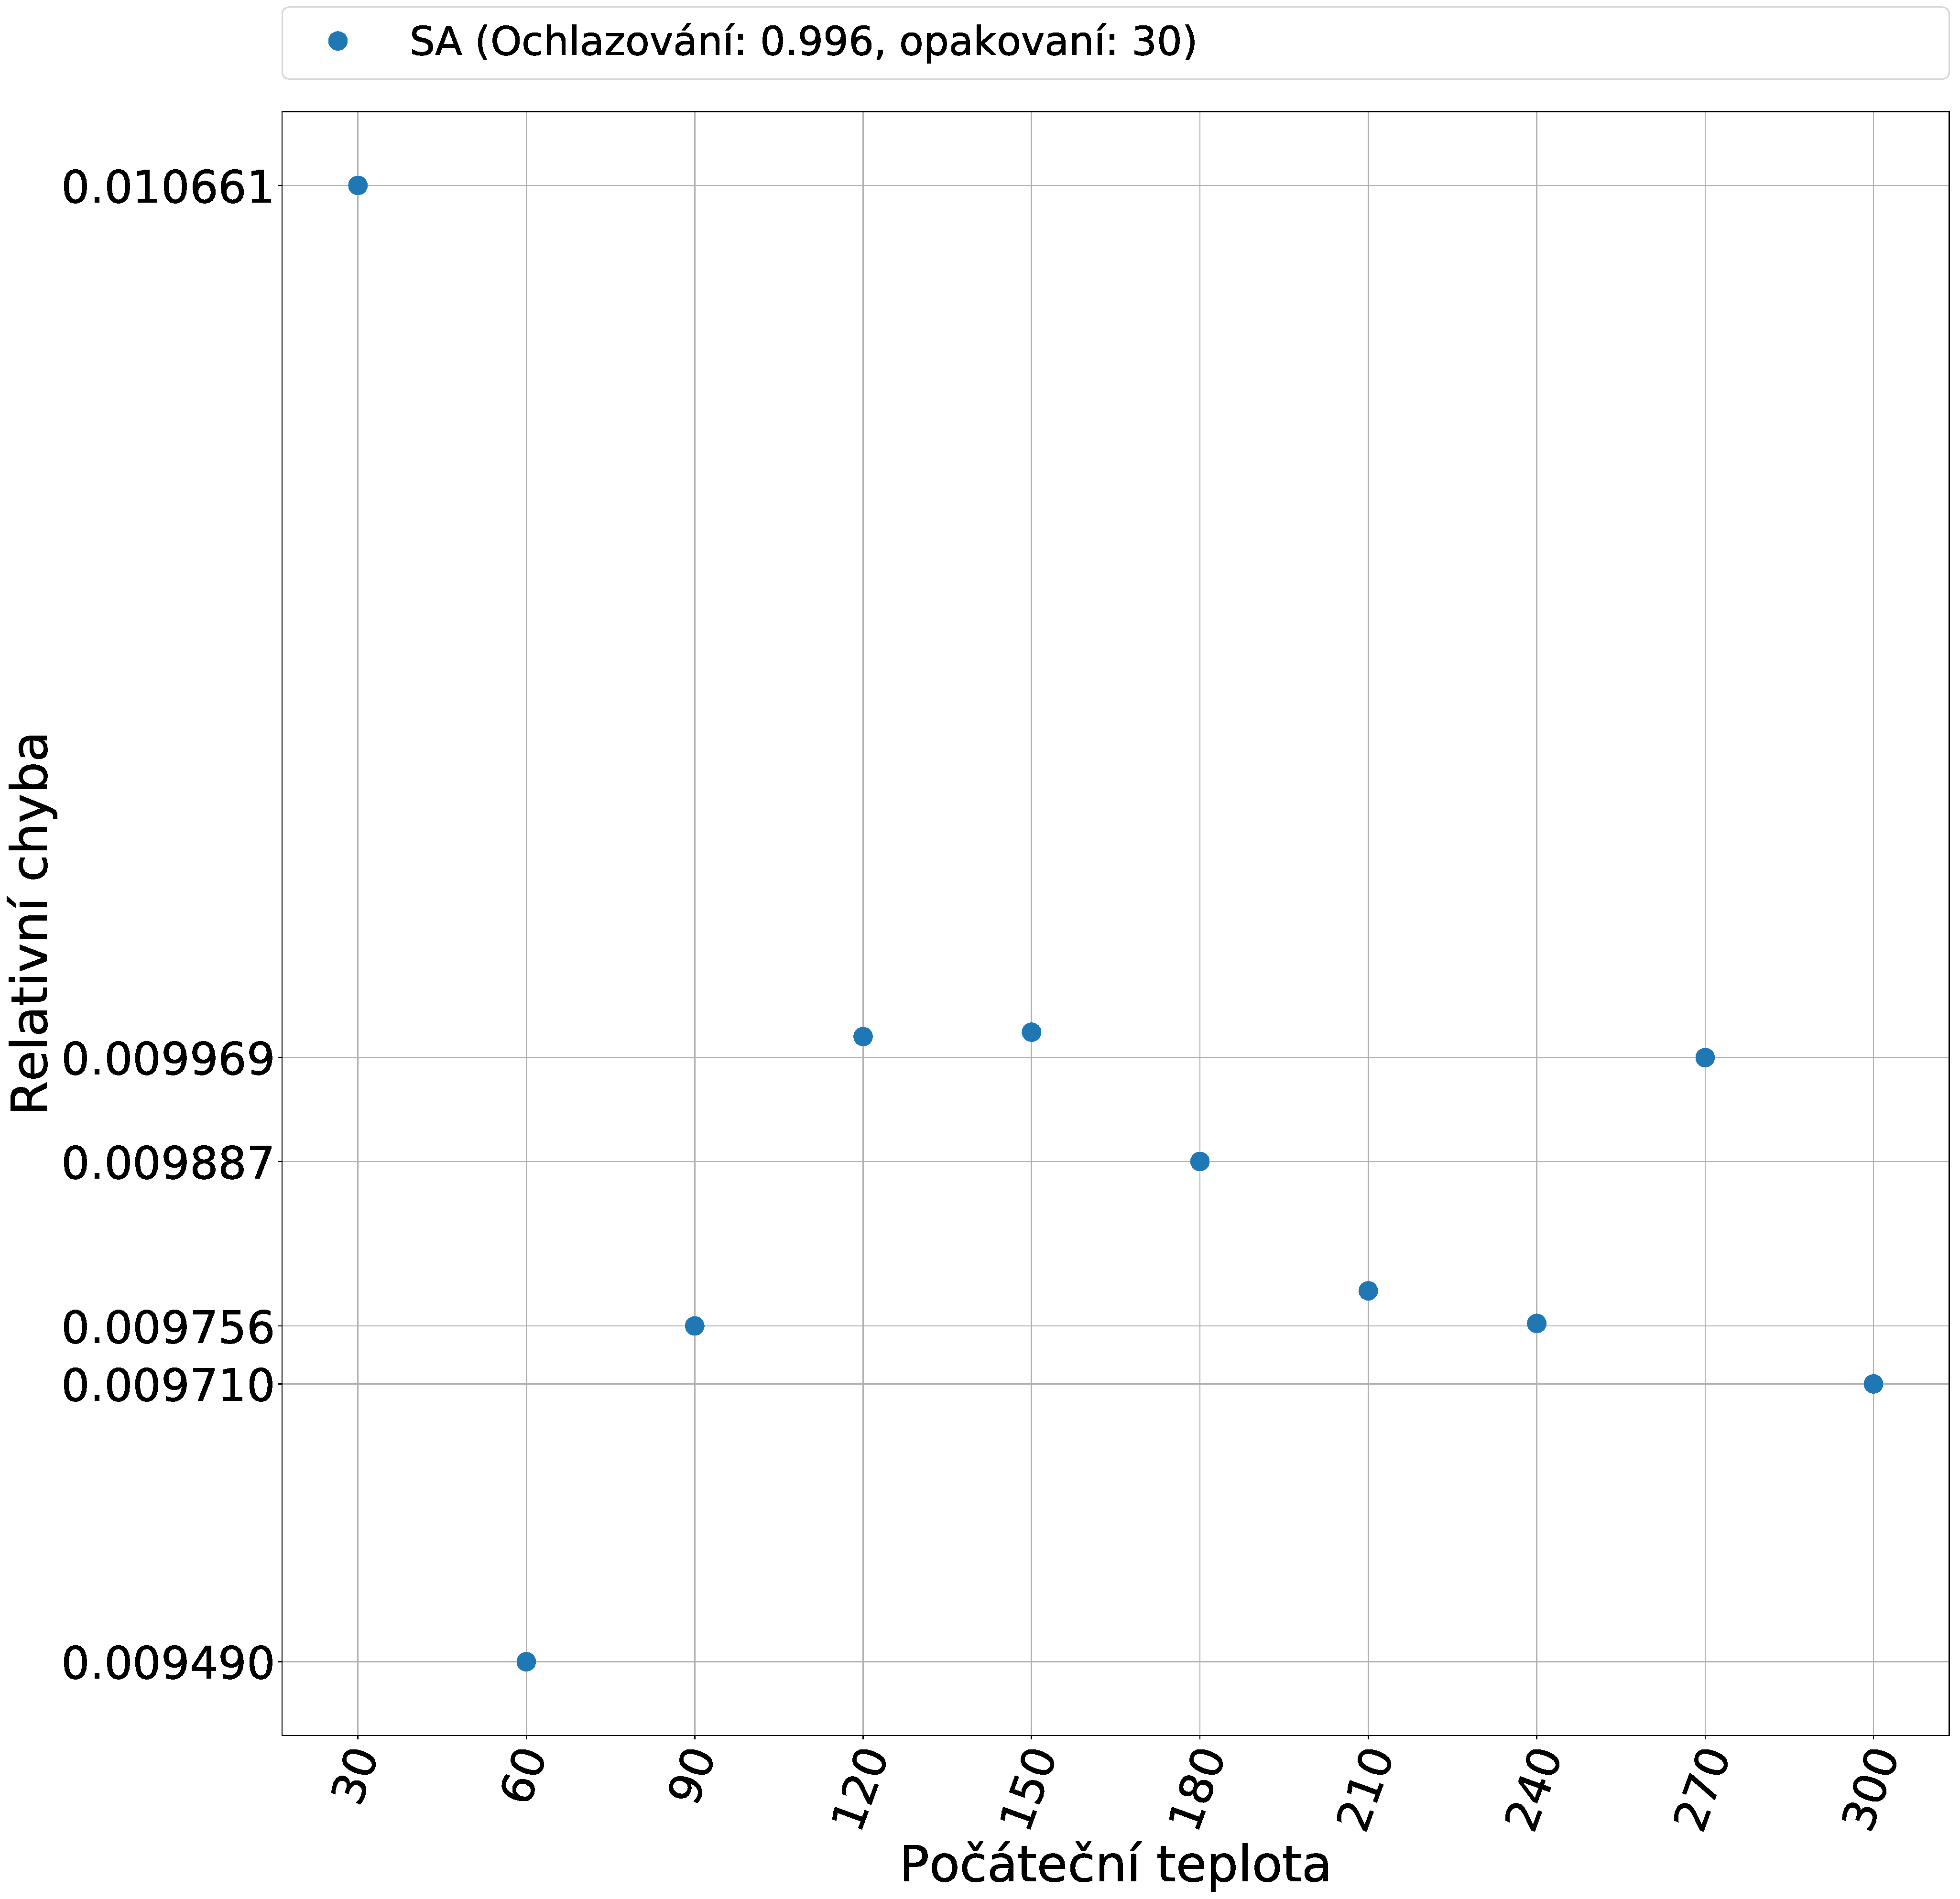
\includegraphics[width=\textwidth]{img/TE.pdf} 
    \end{minipage}
    \begin{minipage}[c]{0.42\textwidth}
        \centering 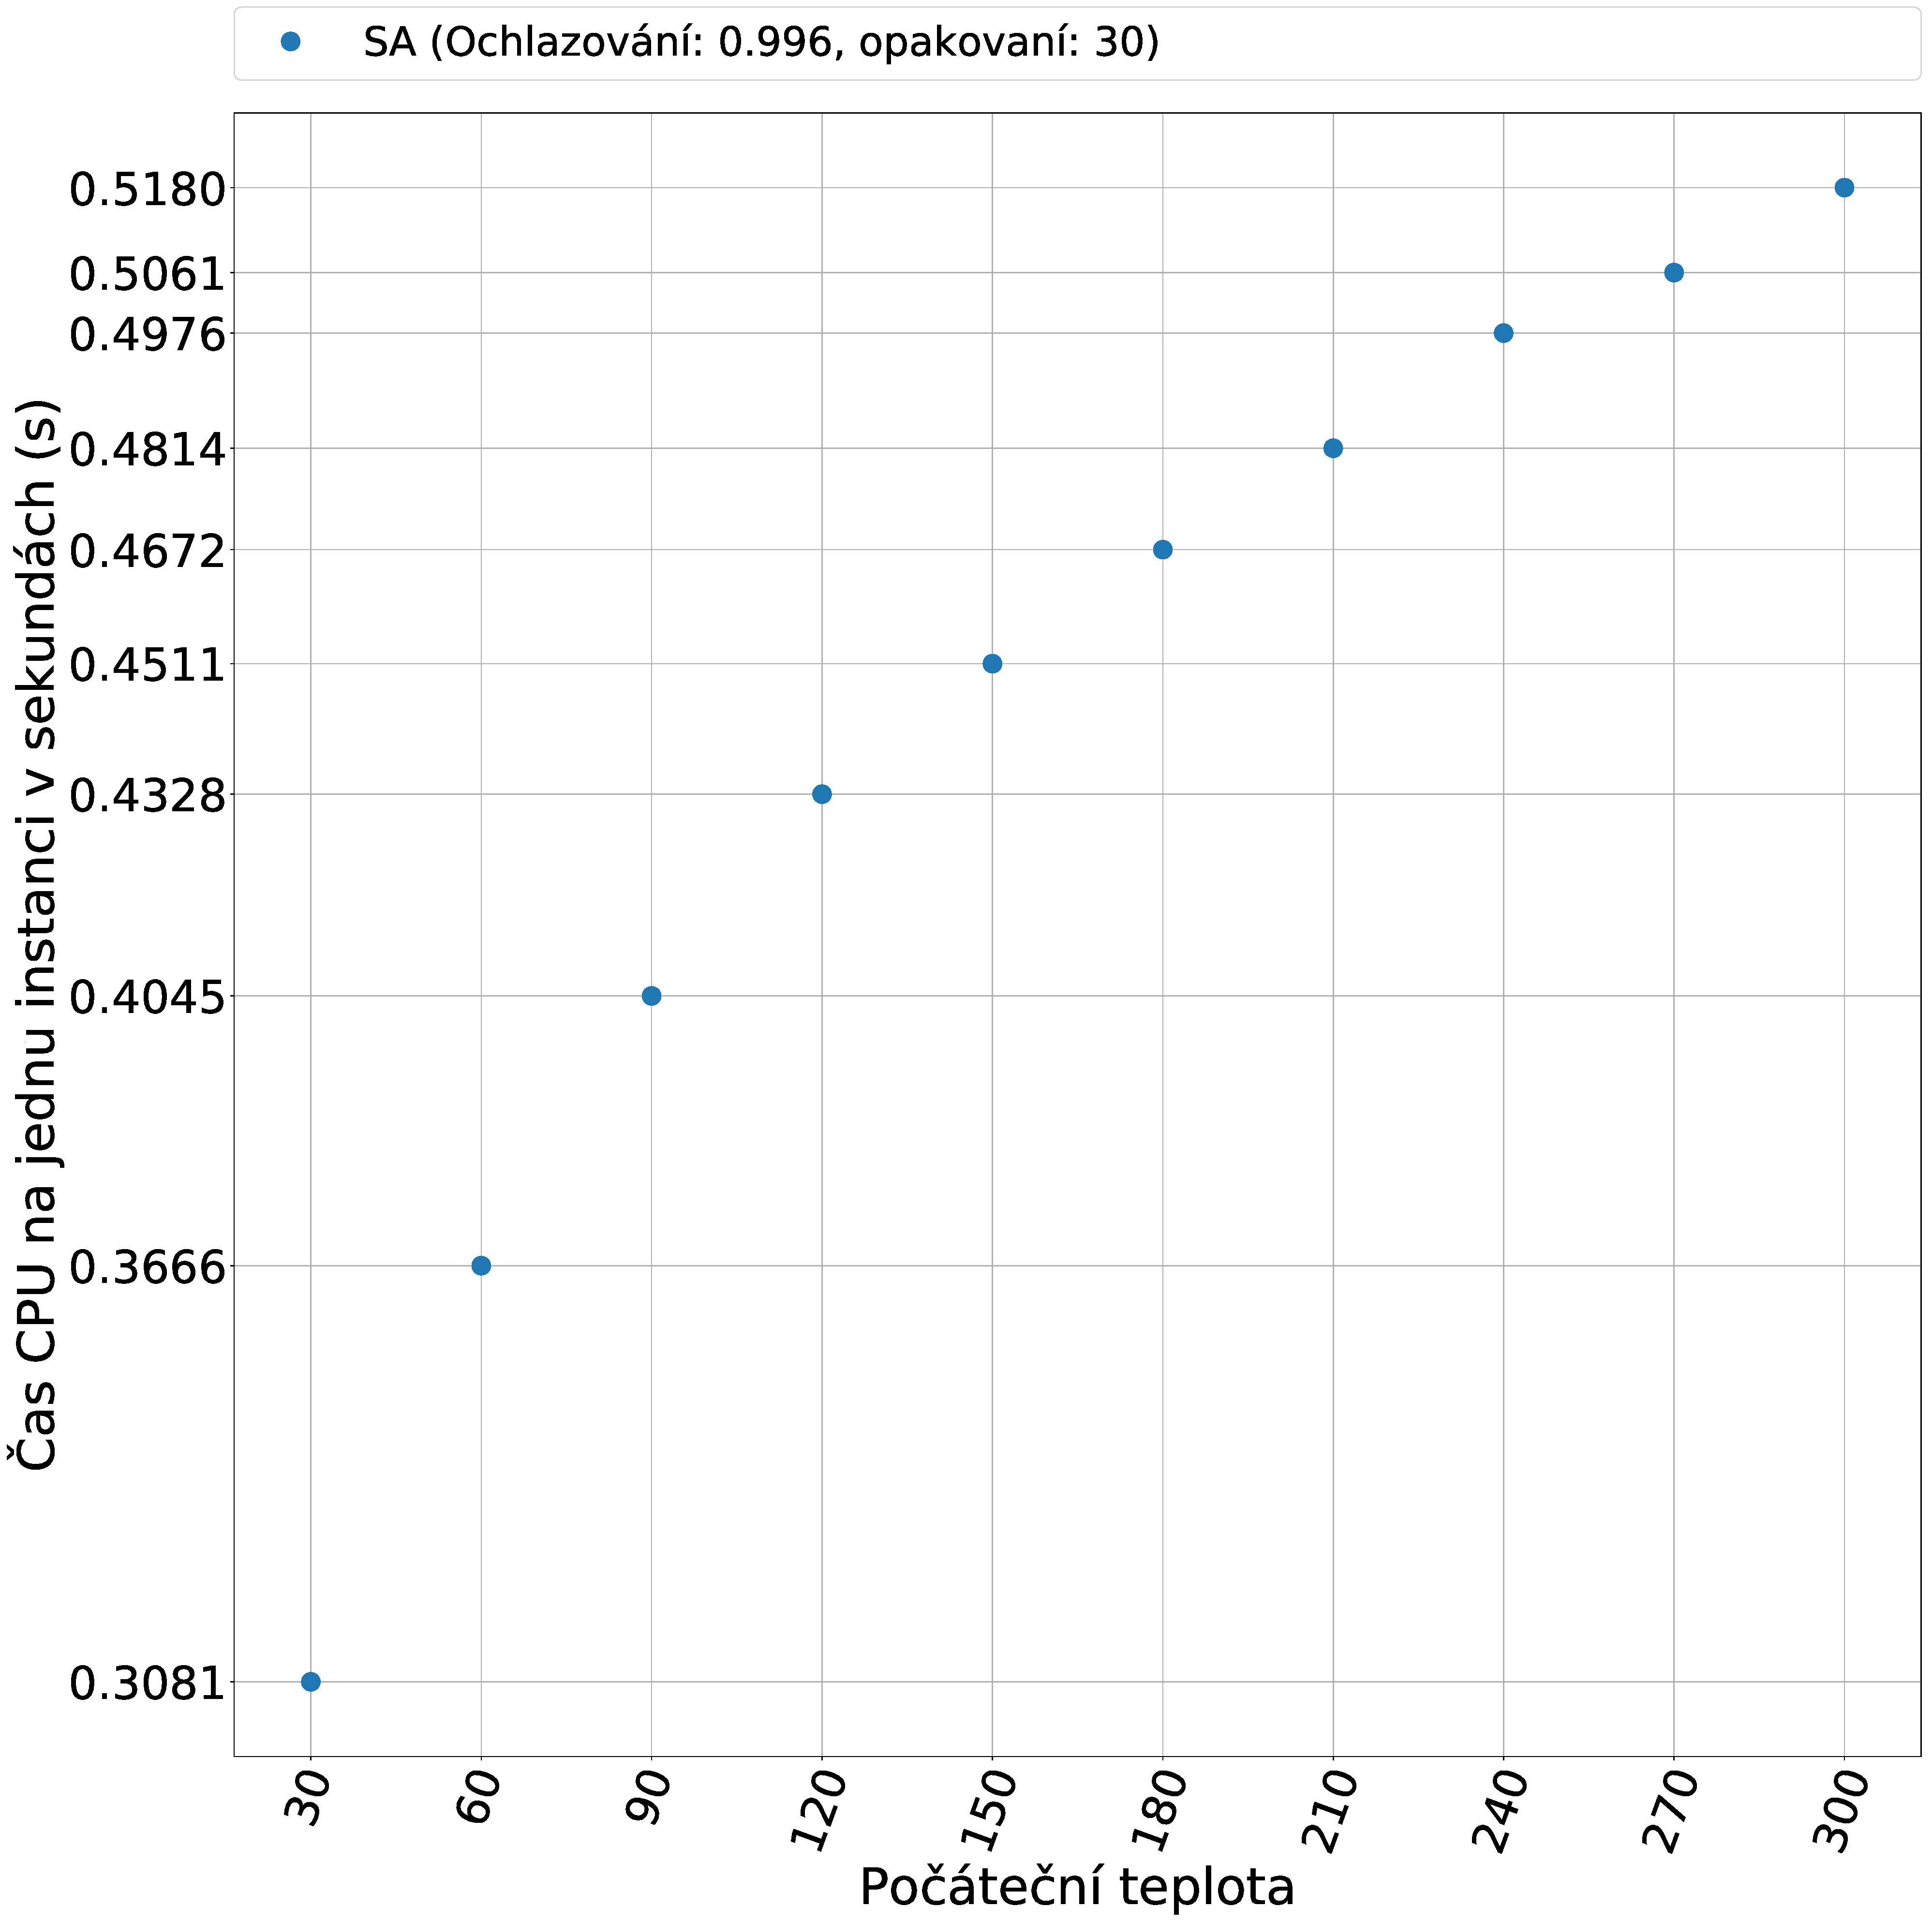
\includegraphics[width=\textwidth]{img/TT.pdf} 
    \end{minipage}
    \\
   \caption{Na levém grafu je závislost relativní chyby na počáteční teplotě. Na pravém grafu je závislost výpočetního času na počáteční teplotě}\label{fig:GZNT}
\end{figure} 

\begin{figure}
	\centering
    \begin{minipage}[c]{0.325\textwidth}
        \centering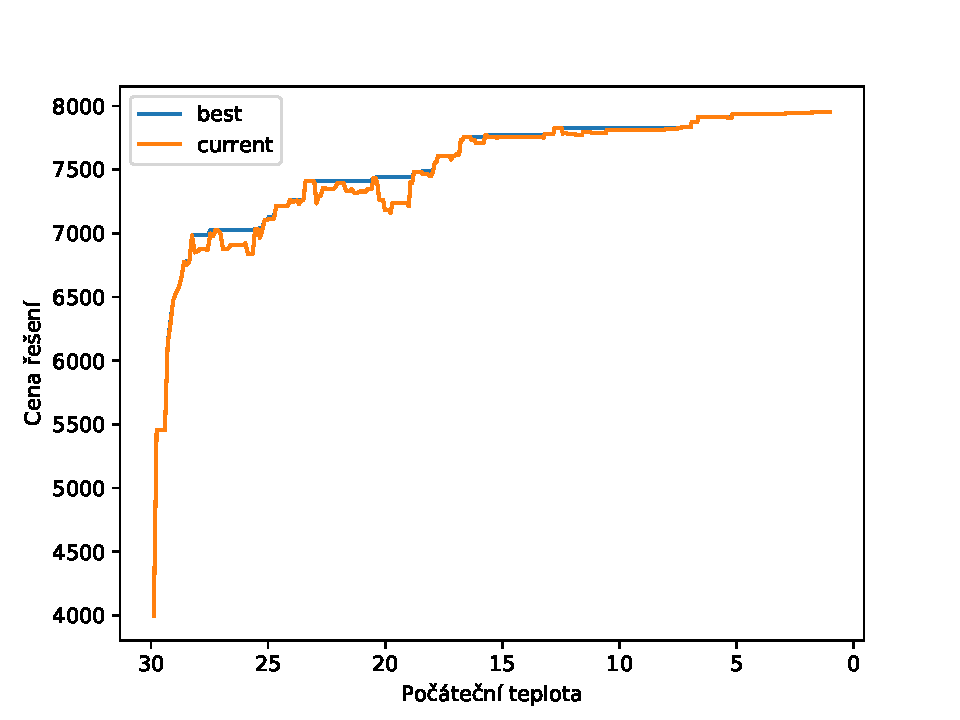
\includegraphics[width=\textwidth]{img/T30.pdf} 
    \end{minipage}
    \begin{minipage}[c]{0.325\textwidth}
        \centering 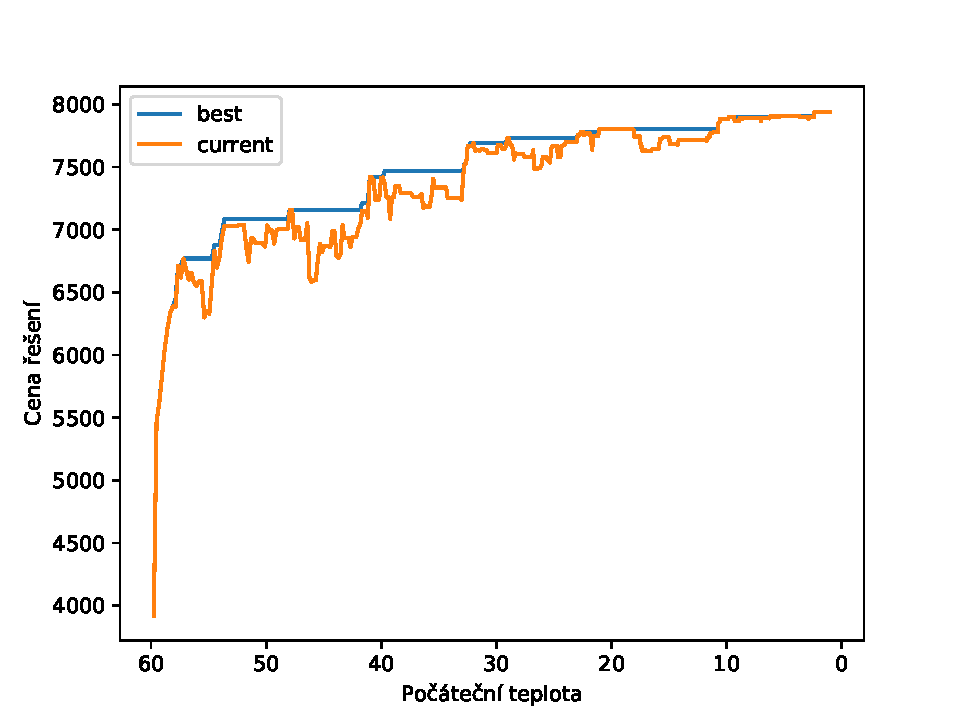
\includegraphics[width=\textwidth]{img/T60.pdf} 
    \end{minipage}
    \begin{minipage}[c]{0.325\textwidth}
        \centering 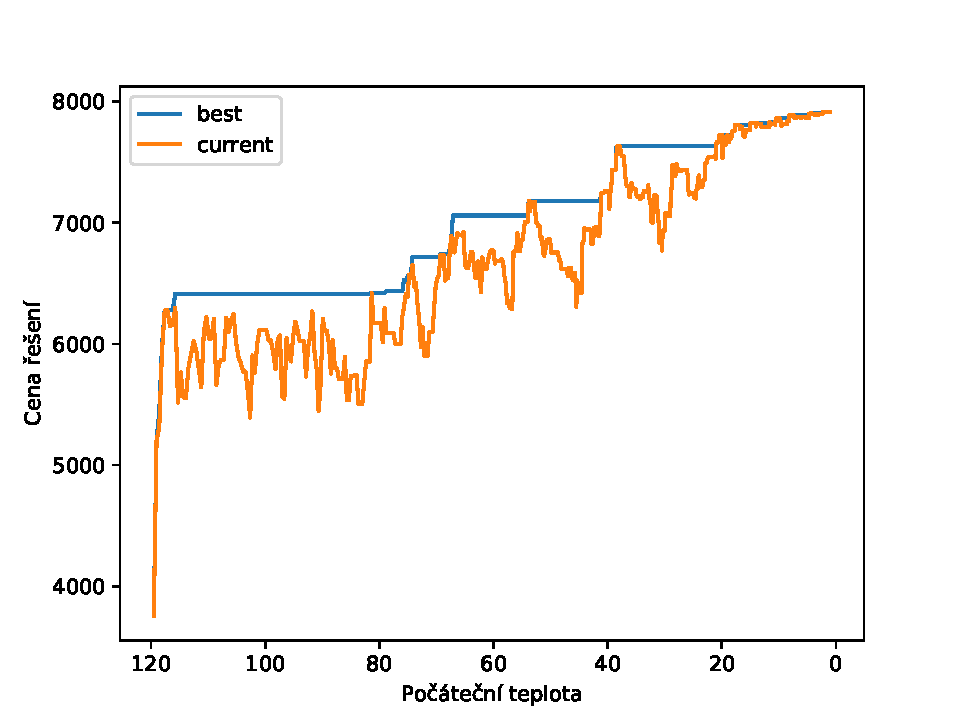
\includegraphics[width=\textwidth]{img/T120.pdf} 
    \end{minipage}
    \\
    \begin{minipage}[c]{0.49\textwidth}
        \centering 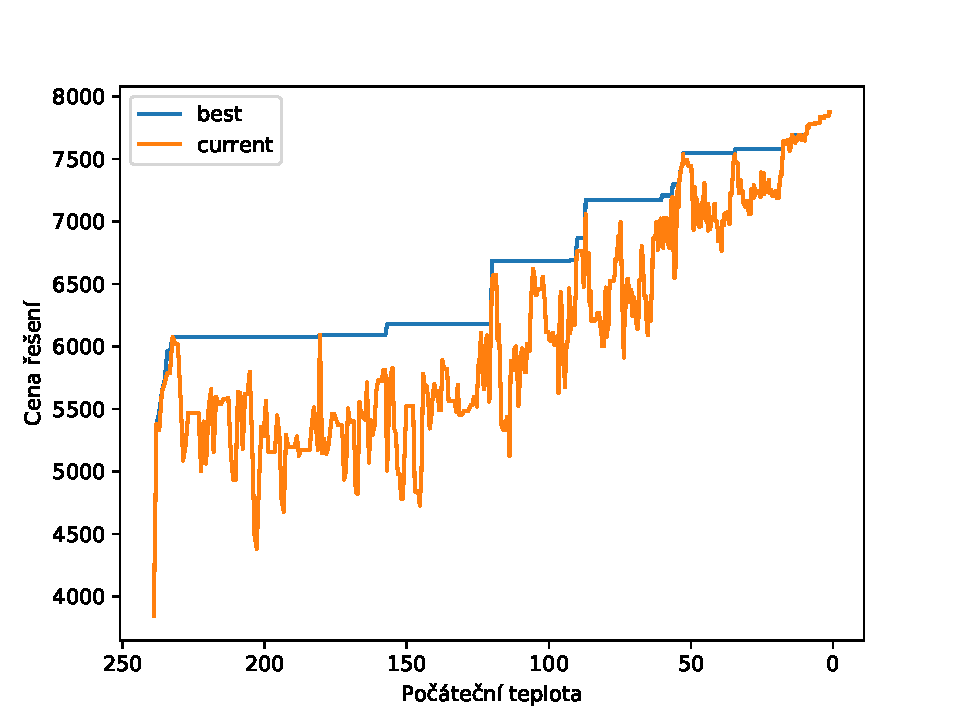
\includegraphics[width=\textwidth]{img/T240.pdf} 
    \end{minipage}
    \begin{minipage}[c]{0.49\textwidth}
        \centering 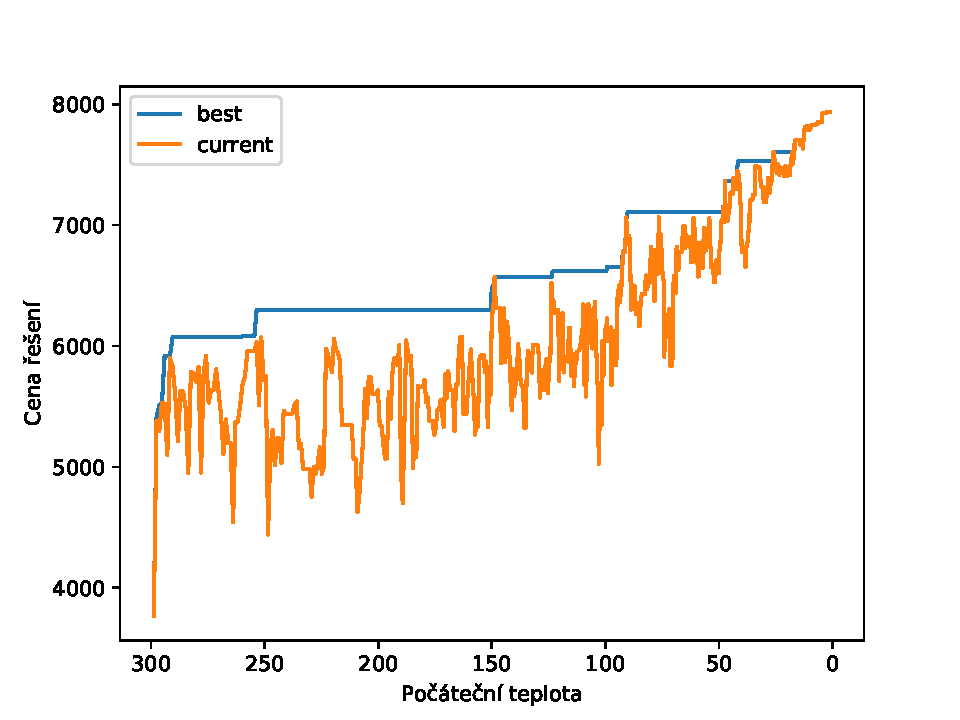
\includegraphics[width=\textwidth]{img/T300.pdf} 
    \end{minipage}
   \caption{Zde jsou uvedené grafy vývoje řešení pro vybrané hodnoty počtu iterácí na jedné teplotě. Konkrétně zleva pro hodnoty 30, 60, 120, 240, 300}\label{fig:GVPT}
\end{figure} 

Nejprve jsem zkoumal chování simulovaného ochlazování v závislosti na počáteční teplotě. Odhadoval jsem, že s rostoucí počáteční teplotou bude klesat relativní chyba a poroste výpočetní náročnost. 

Z grafů \ref{fig:GZNT} je vidět, že relativní chyba nemá patrný odhadováný trend v závislosti na počáteční teplotě. Je zde pouze vysoká chyba pro nízkou počáteční hodnotu, která může být způsobena nízkým počtem kroků algoritmu. Počáteční teplota tedy ovlivňuje počet kroků, které algoritmus provede, ale také dává velkou pravněpodobnost přijetí zhoršujícího se řešení, protože z kapitoly \ref{kap:1} a vzorce pro výpočet pravděpodobnosti zde teplota přímo vystupuje. 

Při pohledu na graf závisloti na výpočetním čase je vidět, že závilost je menší než lineární. To je dána schématem ochlazování, kdy se vždy aktuální teplota násobí koeficientem ochlazování čímž vzniká nová teplota. 

Na grafu \ref{fig:GVPT} je vývoj nejlepšího a průměrného řešení v závislosti na počáteční teplotě. Při nízké teplotě je patrné, že se průměrné řešení blízko maximálního a~algoritmus tedy nepřijímá příliž zhoršující rešení a bude mít tendence konvergovat do lokálních optim. Se zvyšující teplotou rostla diverzifikační fáze ná počátku, kde bylo velmi často příjímáno zhoršující řešení a~fáze intenzifikace je parná až při snižení teploty ke konci, kde však již může být příliž málo kroků ke konvergenci k~nějakému minimu. 

Volba teploty je tedy velmi důležitá, ale ne vždy platí, že výšší teplota znamená i~lepší výkonost algoritmu, ale hodnota je důležitá ve vzorci pro přijetí zhoršujícího se řešení. V~tomto vzorci také vystupuje rozdíl cen, tedy vyšší teploty mohou být vhodné při výšších hodnotách cen předmentů a~naopak. Výkonost bude záležet i~na dalších parametrech a závislost parametru mezi sebou sepíši v~závěru.

\subsection{Závislost na koeficientu ochlazování}
\begin{figure}
	\centering
    \begin{minipage}[c]{0.42\textwidth}
        \centering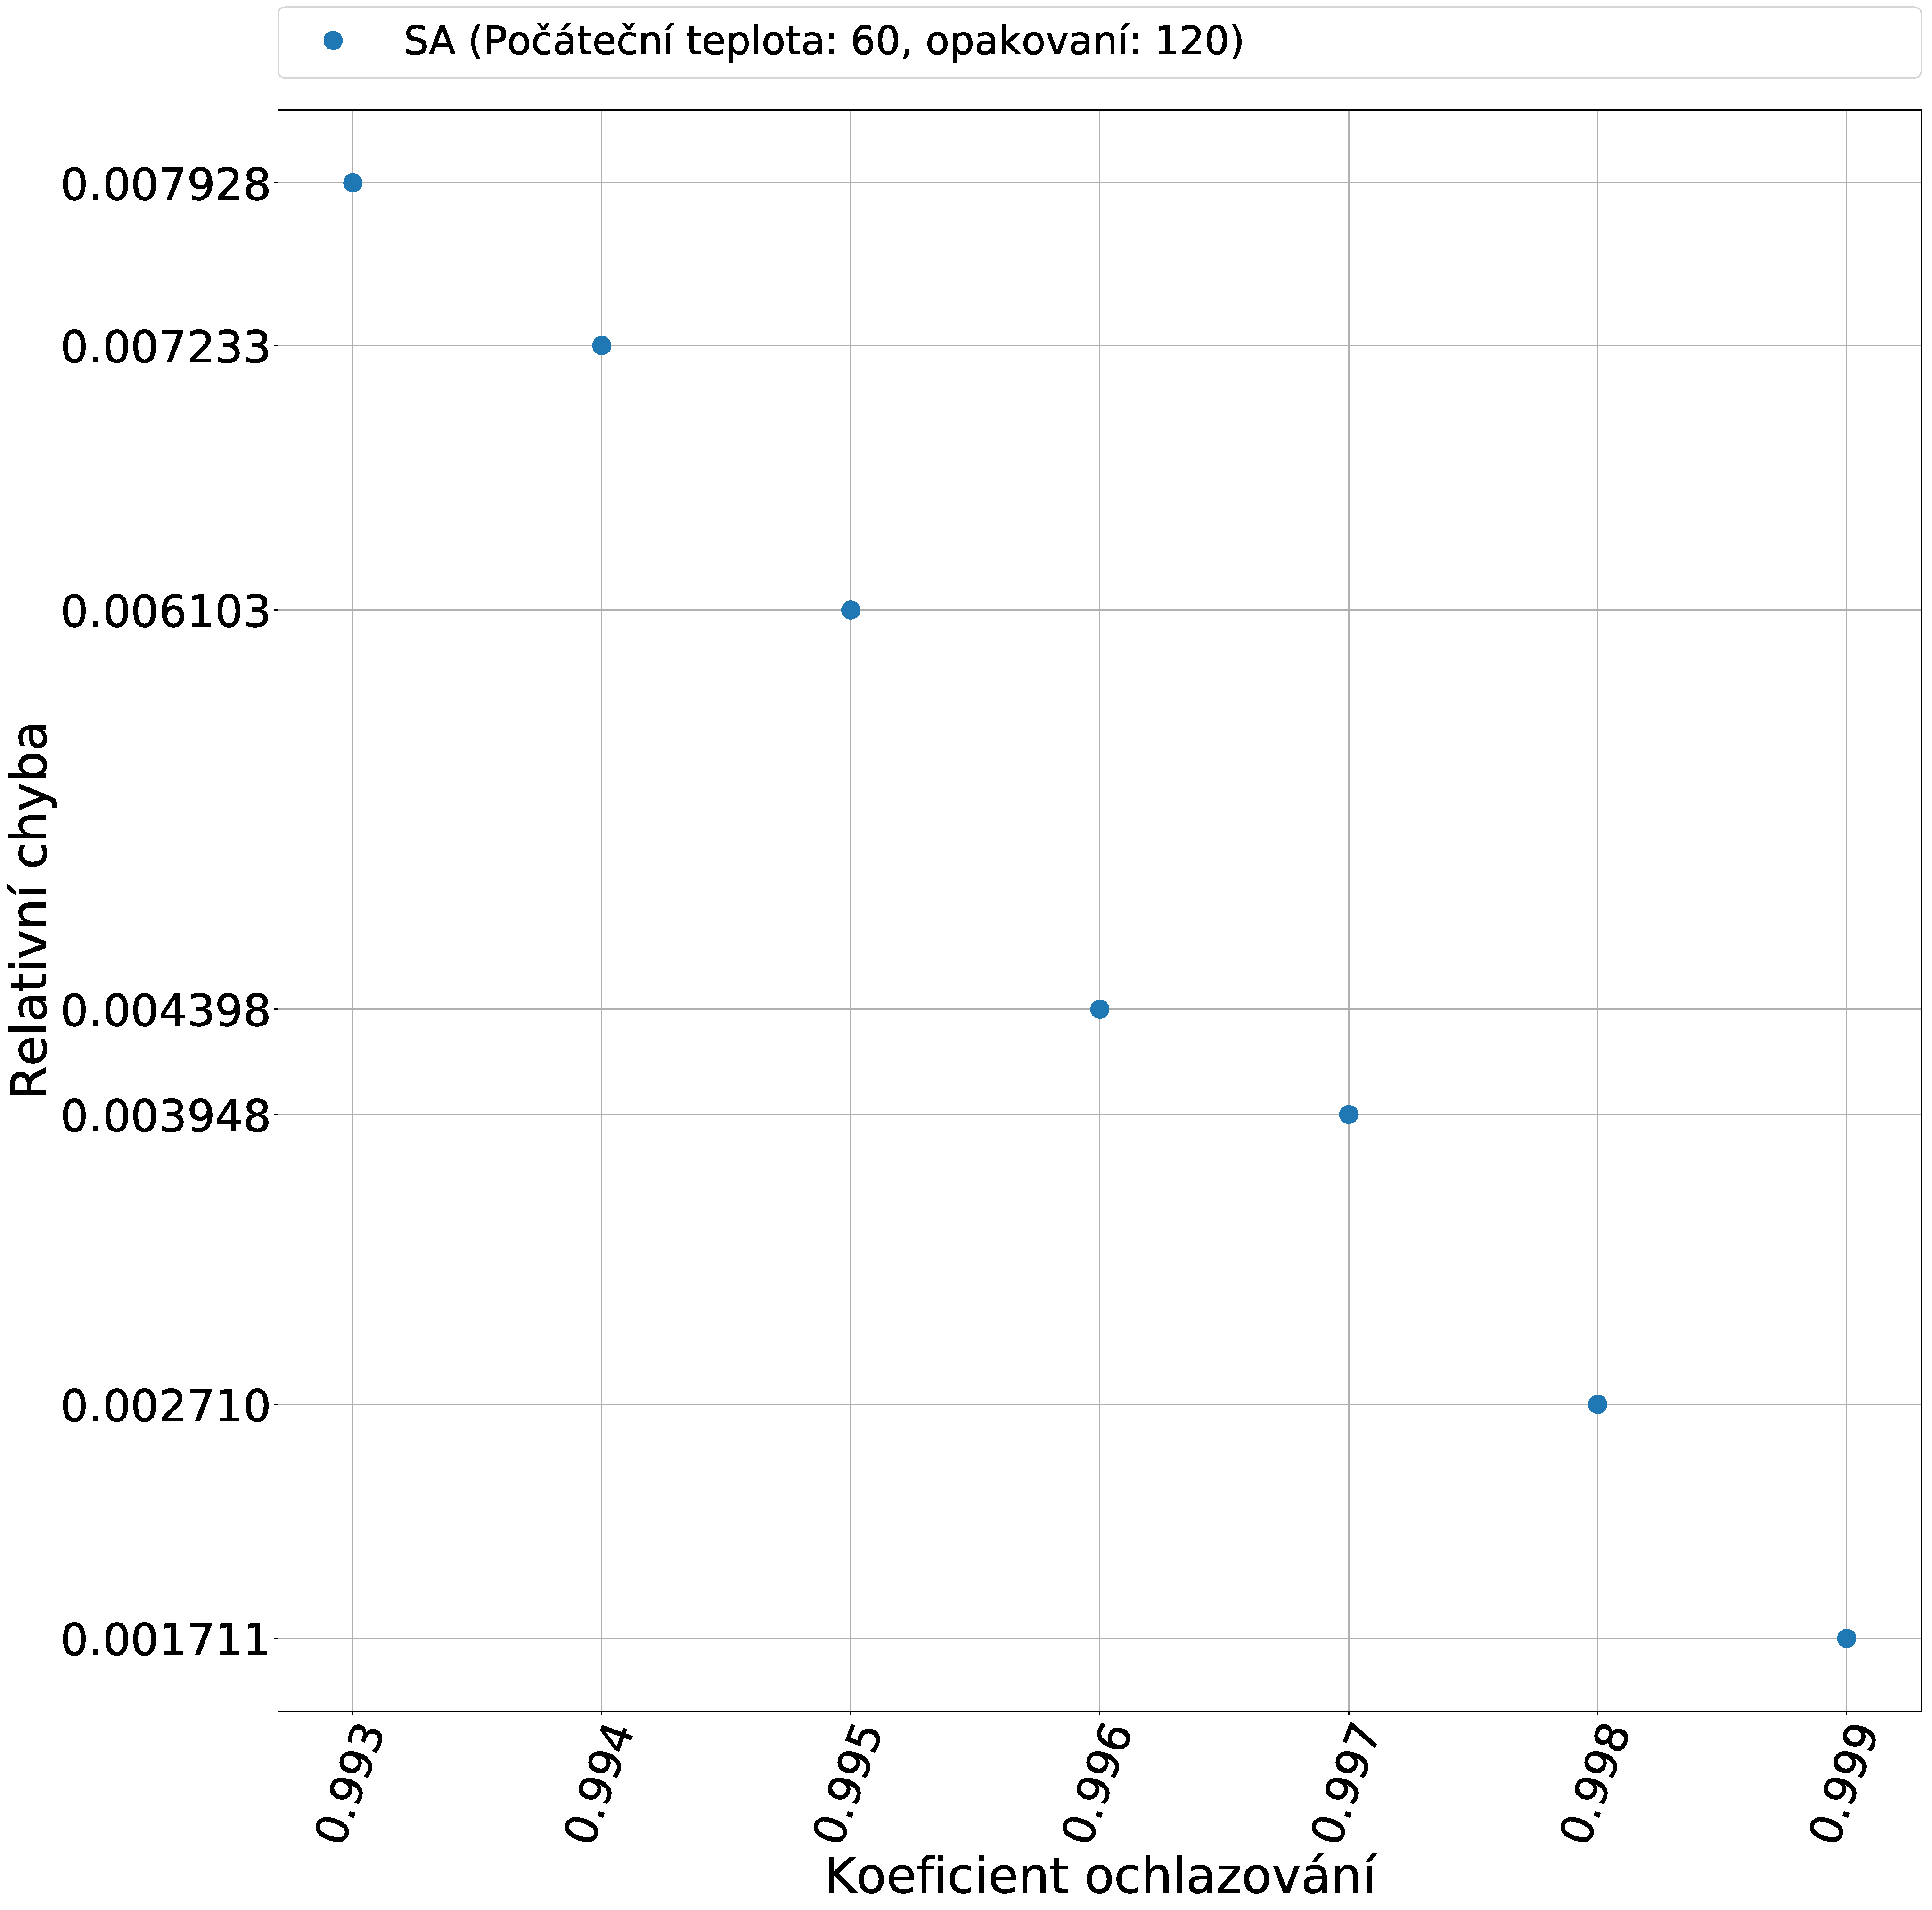
\includegraphics[width=\textwidth]{img/KE.pdf} 
    \end{minipage}
    \begin{minipage}[c]{0.42\textwidth}
        \centering 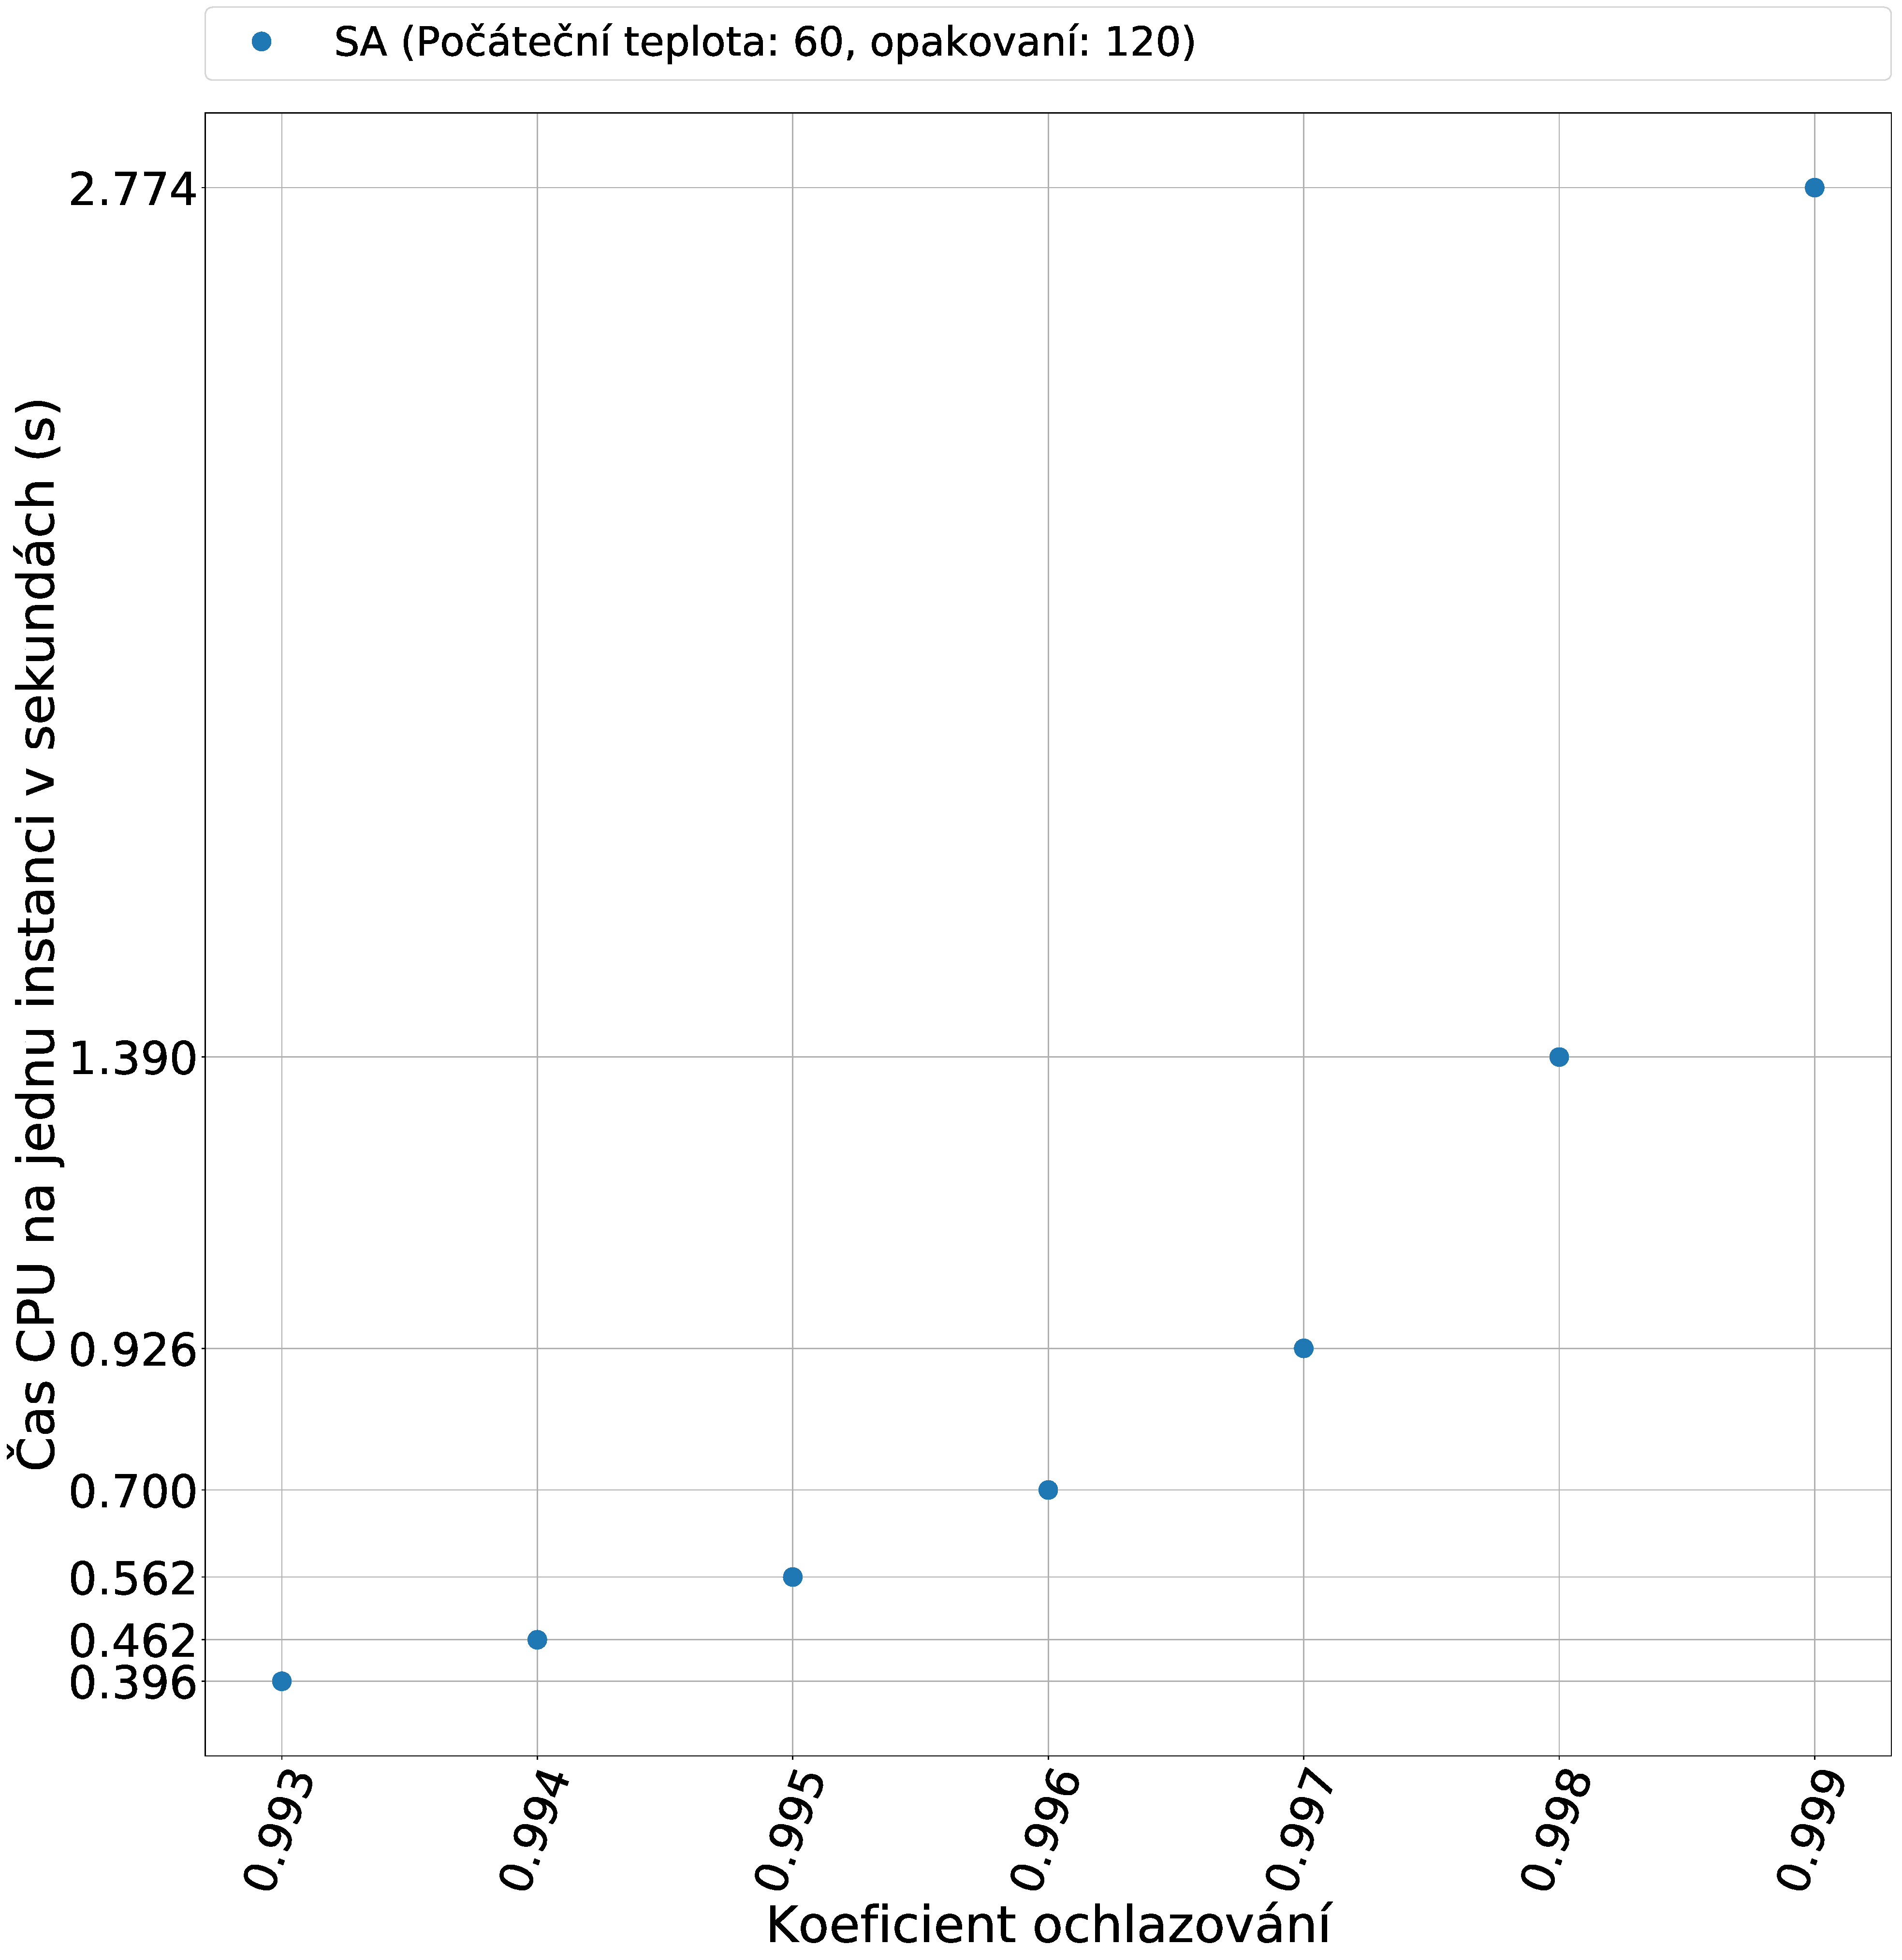
\includegraphics[width=\textwidth]{img/KT.pdf} 
    \end{minipage}
    \\
   \caption{Na levém grafu je závislost relativní chyby na koeficientu ochlazování. Na pravém grafu je závislost výpočetního času na koeficientu ochlazování}\label{fig:GZNK}
\end{figure} 




\begin{figure}
	\centering
    \begin{minipage}[c]{0.48\textwidth}
        \centering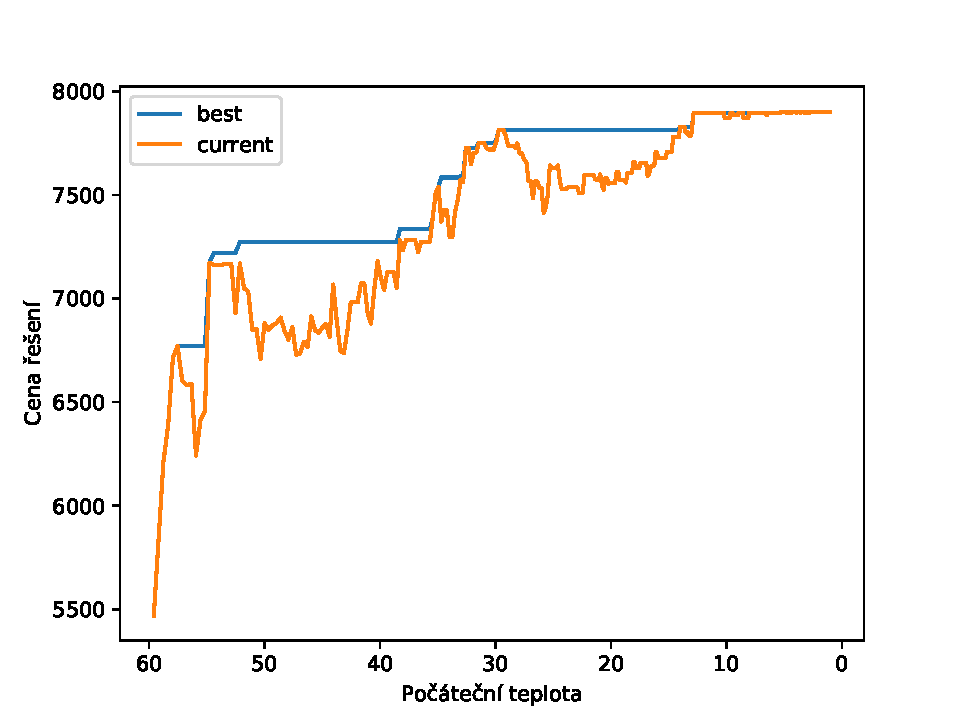
\includegraphics[width=\textwidth]{img/993.pdf} 
    \end{minipage}
    \begin{minipage}[c]{0.48\textwidth}
        \centering 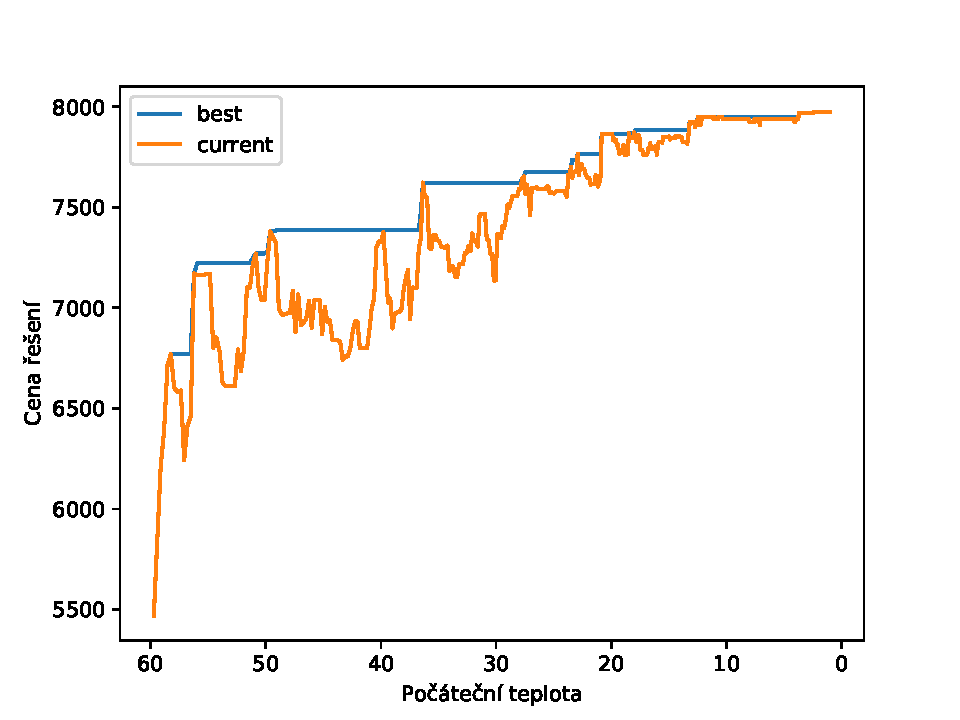
\includegraphics[width=\textwidth]{img/995.pdf} 
    \end{minipage}
    \\
    \begin{minipage}[c]{0.48\textwidth}
        \centering 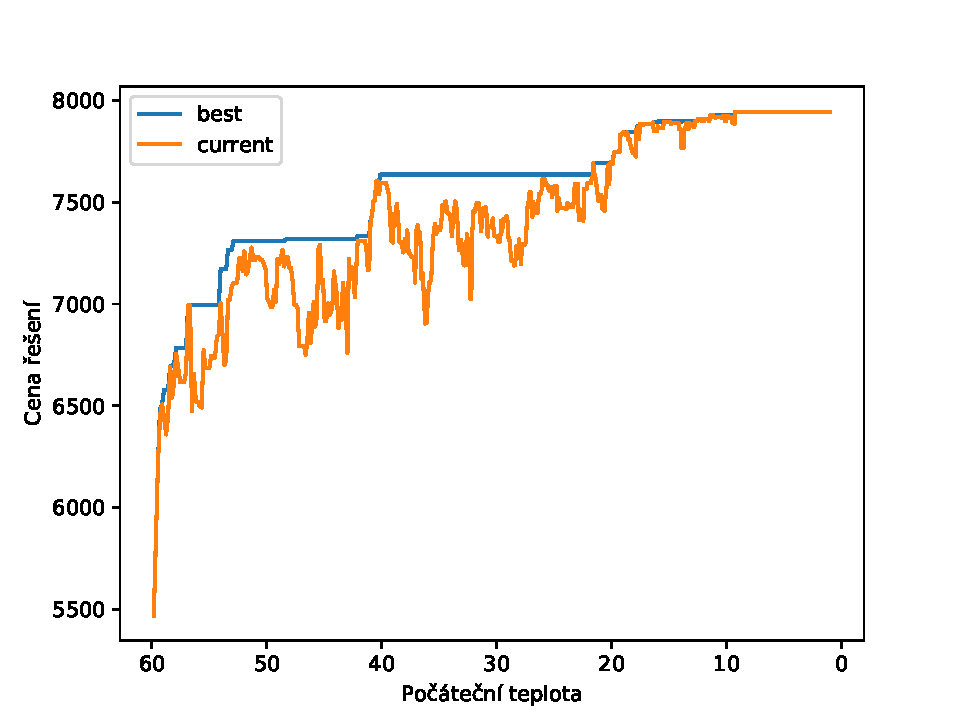
\includegraphics[width=\textwidth]{img/997.pdf} 
    \end{minipage}
    \begin{minipage}[c]{0.48\textwidth}
        \centering 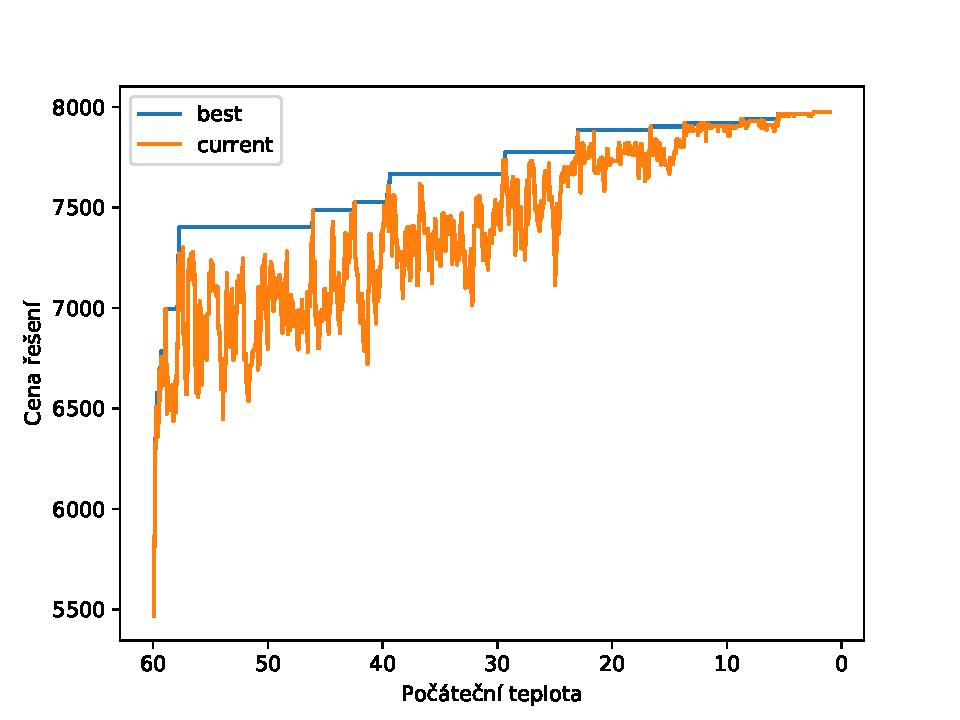
\includegraphics[width=\textwidth]{img/999.pdf} 
    \end{minipage}
   \caption{Zde jsou uvedené grafy vývoje řešení pro vybrané hodnoty koeficientu ochlazovaní. Konkrétně zleva pro hodnoty 0.993, 0.995, 0.997, 0.999}\label{fig:GVPK}
\end{figure} 

V závislosti na koeficientu ochlazování jsem očekával, že bude klesat relativní chyba s koeficientem blížícím se k hodnotě jedna a zároveň narůstající čas, protože počet kroků roste rychleji než lineárně. 

Při pohldu na grafy \ref{fig:GZNK} se odhad potvrdil. S klesajícím koeficientem klesá relativní chyba lineárně. Čím je koeficient vyšší tím více kroků algoritmus provede, ale počítání vzorce pro přijetí zhoršujícího řešení bude mít pořád stejné hodnoty, potože na koeficientu ochlazování nezávisí. Algoritmus tedy ve fázi intenzifikace s vyšším koeficientem ochlazování provede vyšší počet kroků a prozkoumá větší část okolí a to zvyšuje šanci na nalezení optimálního řešení. 

Na grafe vývoje řešení \ref{fig:GVPK} je toto taky patrné. Výšší počet kroků je vizuálně z grafů patrný. Je vidět, že pro nízké koeficienty ochlazování algoritmus často dokonverguje do lokálního optima brzo. 

Vývoj grafů je velice podobný těm u vývoje teploty, ale u teploty byla více parná fáze diverzifikace, kde se algoritmus pro výsoké teploty nezlepšoval a často přijímal zhršující se řešení. Při zvýšení koeficientu se tento trend neodehrává a zlepšování rešení probíhá plynuleji. 

\subsection{Závislost na počtu iterací na jedné teplotě}
 \begin{figure}
	\centering
    \begin{minipage}[c]{0.42\textwidth}
        \centering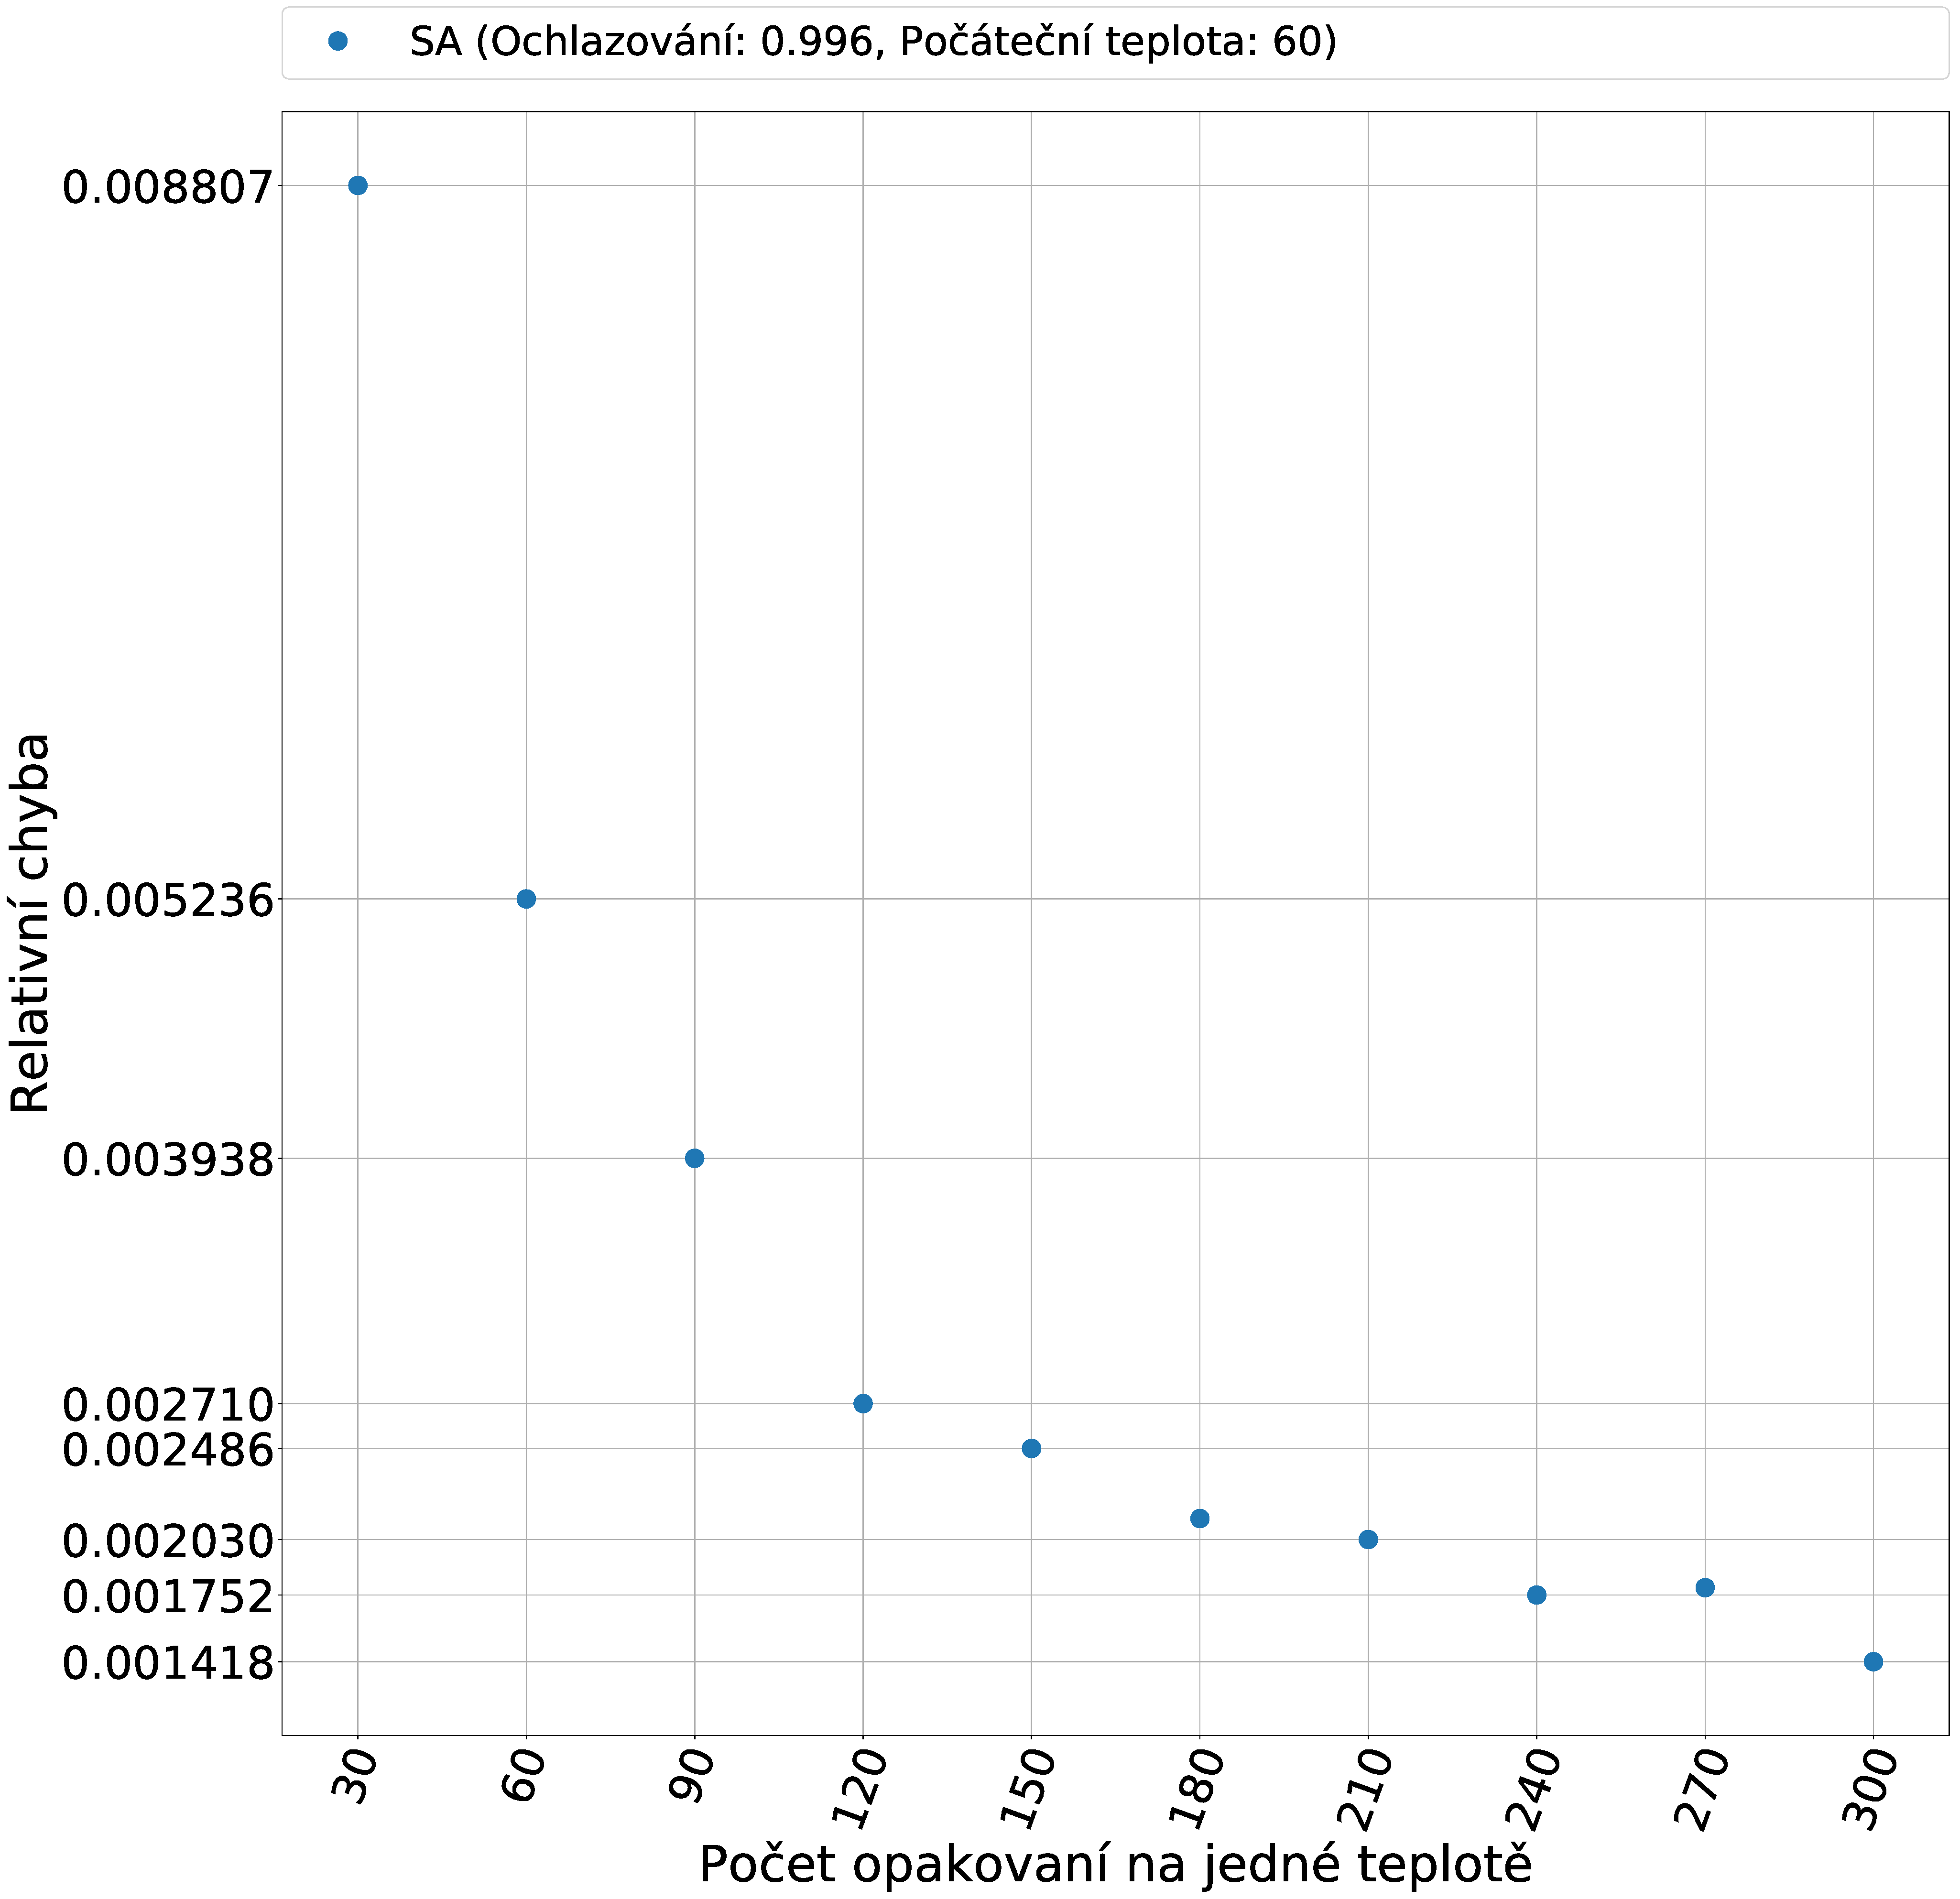
\includegraphics[width=\textwidth]{img/CE.pdf} 
    \end{minipage}
    \begin{minipage}[c]{0.42\textwidth}
        \centering 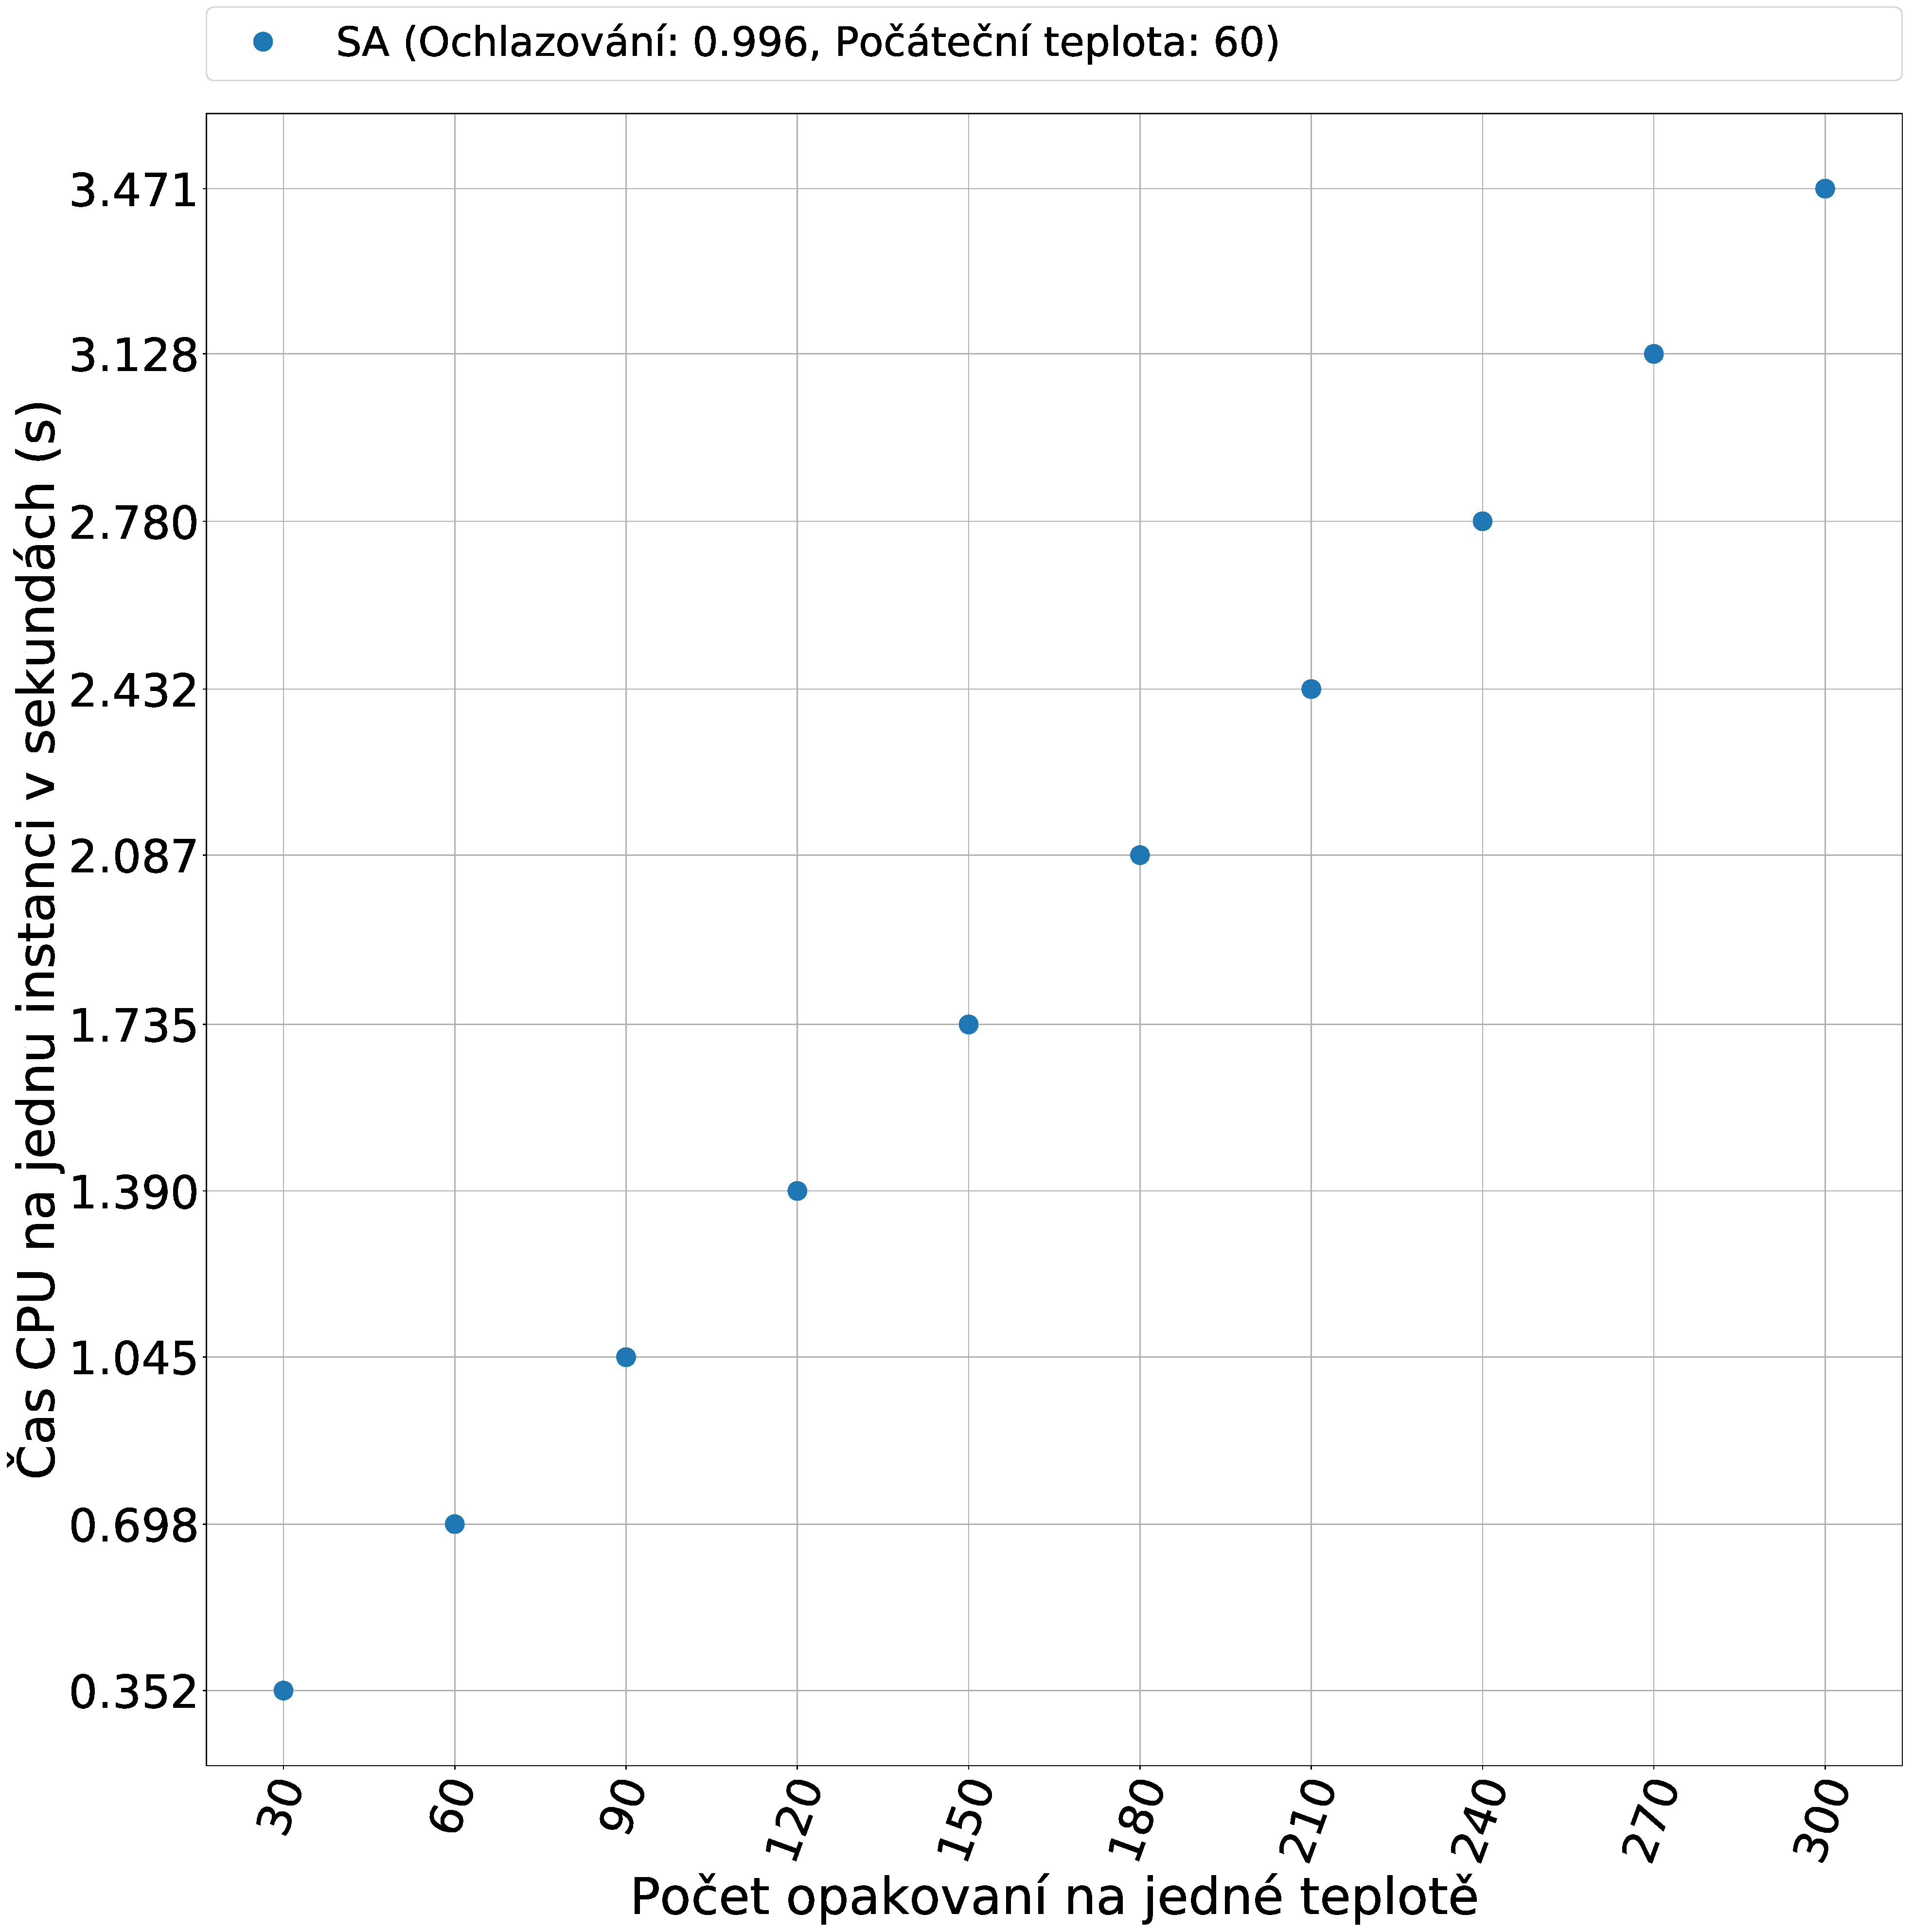
\includegraphics[width=\textwidth]{img/CT.pdf} 
    \end{minipage}
    \\
   \caption{Na levém grafu je závislost relativní chyby na počtu iterací na jedné teplotě. Na pravém grafu je závislost výpočetního času na počtu iterací na jedné teplotě}\label{fig:GZNC}
\end{figure} 

\begin{figure}
	\centering
    \begin{minipage}[c]{0.32\textwidth}
        \centering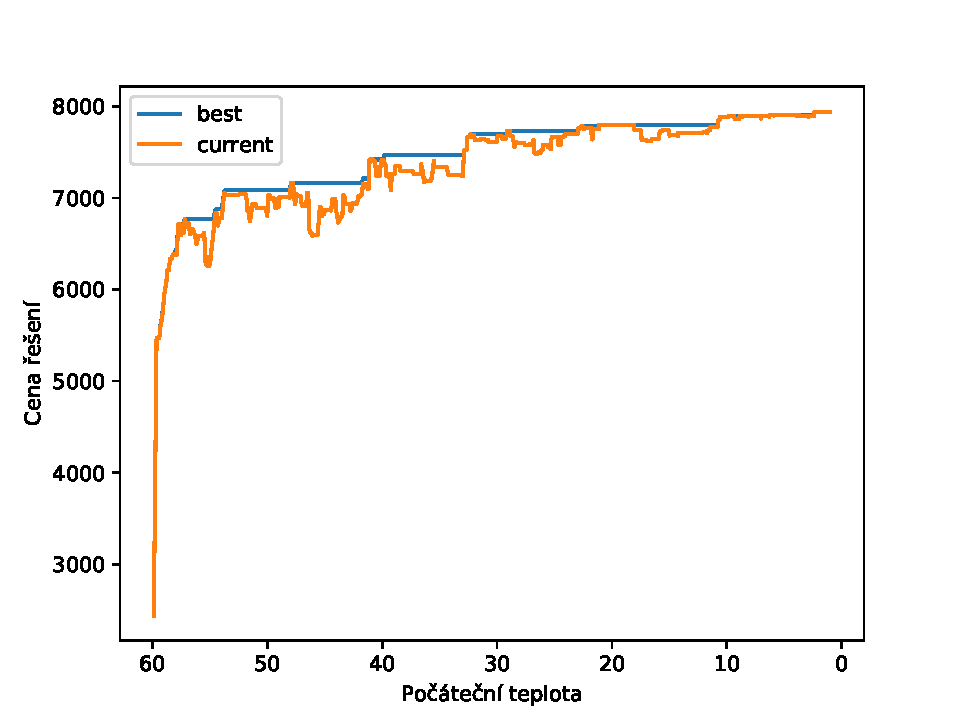
\includegraphics[width=\textwidth]{img/C30.pdf} 
    \end{minipage}
    \begin{minipage}[c]{0.32\textwidth}
        \centering 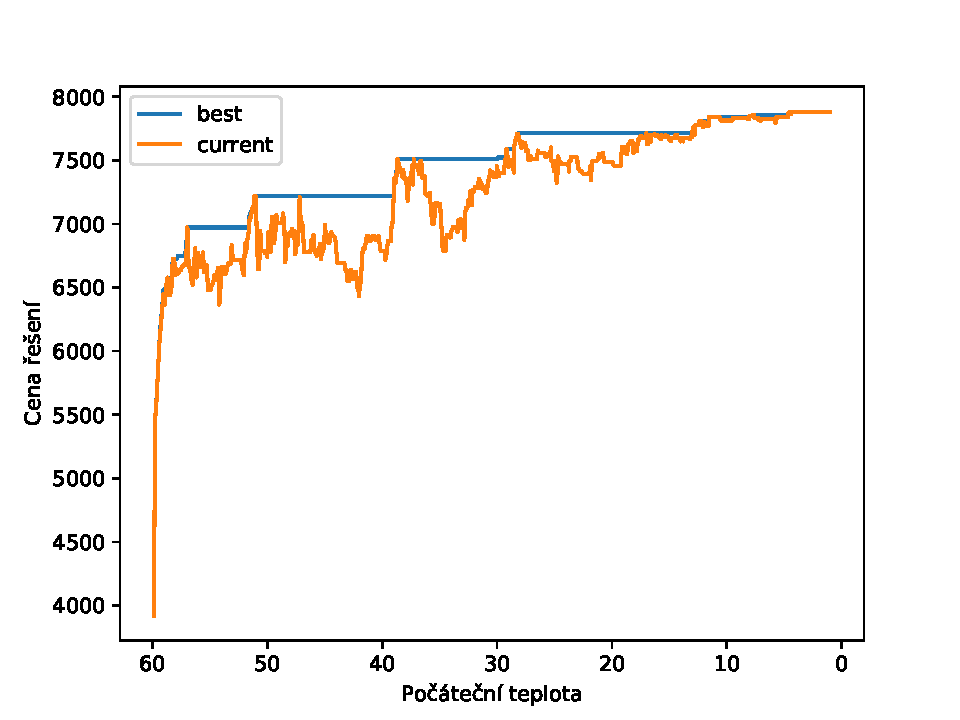
\includegraphics[width=\textwidth]{img/C60.pdf} 
    \end{minipage}
    \begin{minipage}[c]{0.32\textwidth}
        \centering 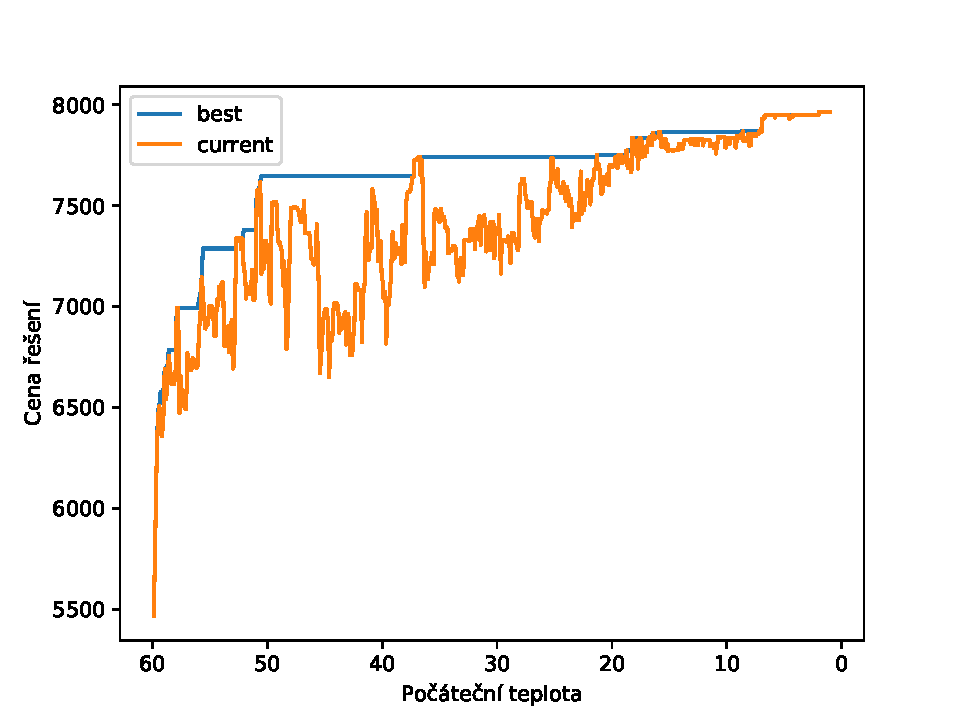
\includegraphics[width=\textwidth]{img/C120.pdf} 
    \end{minipage}
    \\
    \begin{minipage}[c]{0.32\textwidth}
        \centering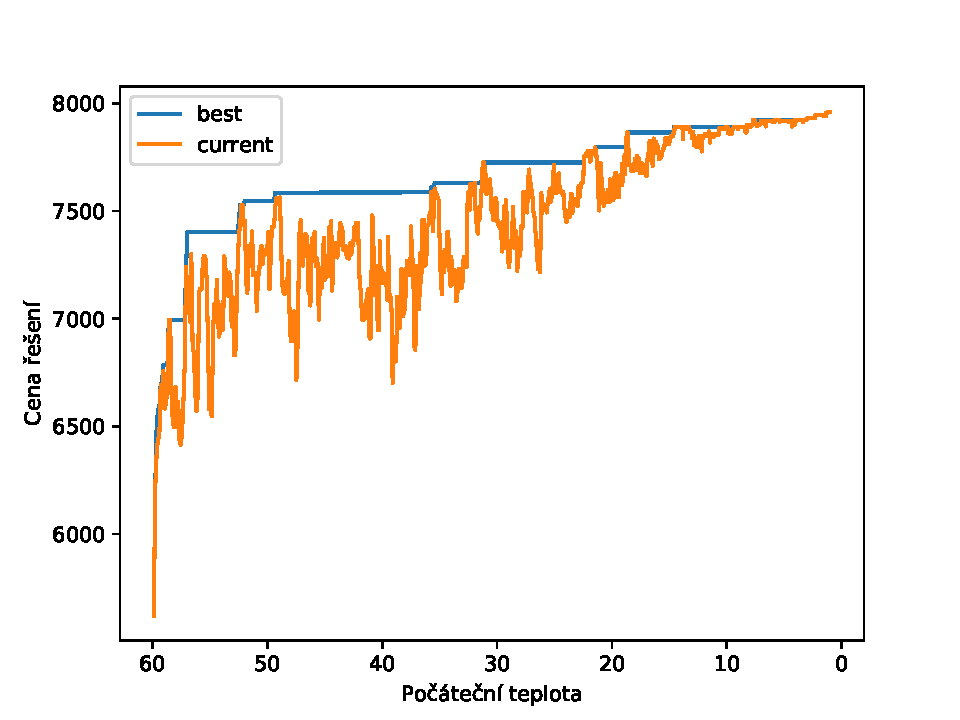
\includegraphics[width=\textwidth]{img/C180.pdf} 
    \end{minipage}
    \begin{minipage}[c]{0.32\textwidth}
        \centering 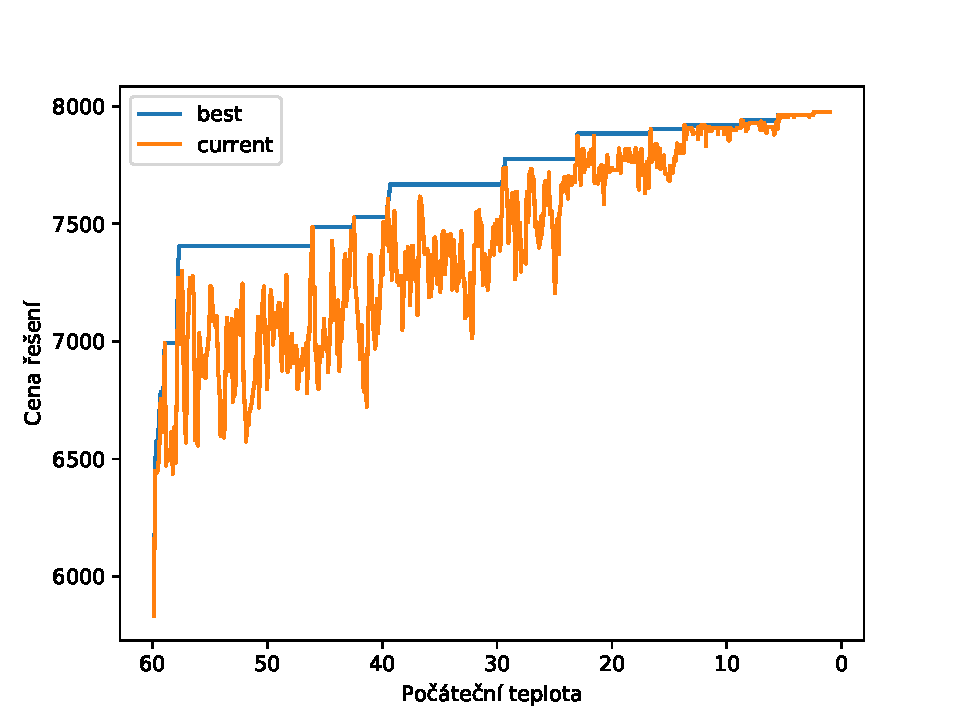
\includegraphics[width=\textwidth]{img/C240.pdf} 
    \end{minipage}
    \begin{minipage}[c]{0.32\textwidth}
        \centering 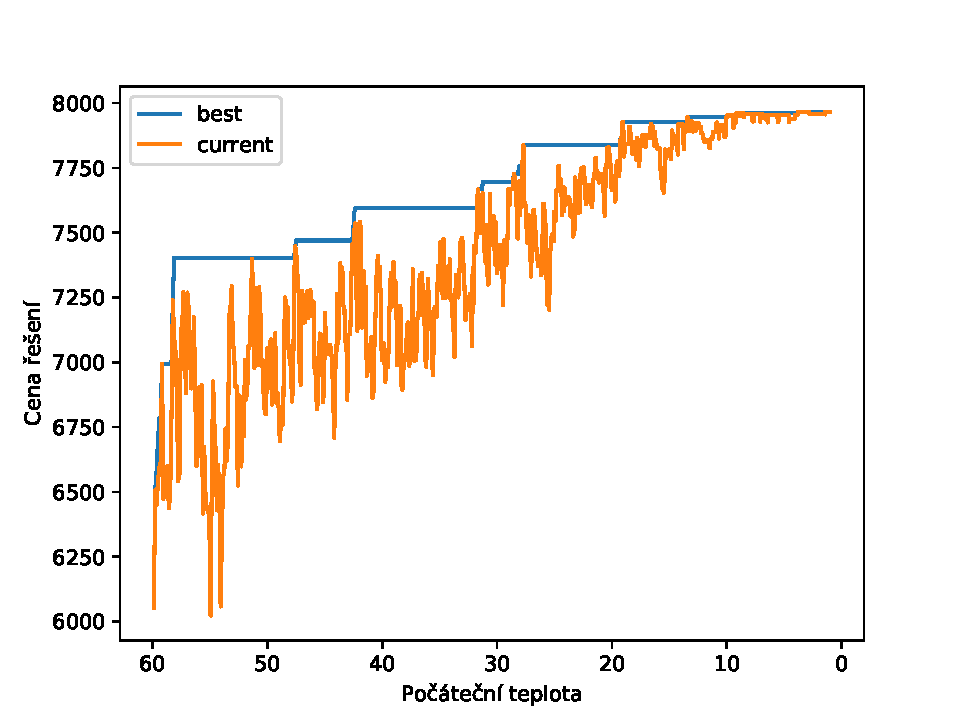
\includegraphics[width=\textwidth]{img/C300.pdf} 
    \end{minipage}
   \caption{Zde jsou uvedené grafy vývoje řešení pro vybrané hodnoty počtu iterácí na jedné teplotě. Konkrétně zleva pro hodnoty 30, 60, 120, 180, 240, 300}\label{fig:GVPC}
\end{figure} 

Posledním sledováným parametrem byl počet iterací na jedné hodnotě dané teploty. Odhad je, že by relativní chyba měla klesat, protože je prozkoumáno větší okolí behem jedné iterace a zároveň čas by měl růst lineárně.
  
Odhady se opět potvrdily měřením jak je možno vidět na grafech \ref{fig:GZNC}. Relativní chyba s roustoucím počtem iterací klesala, ovšem ne lineárně, ale po hyperbole. Je tedy možné v závislosti na čase uvažovat o zvolení vhodného počtu iterací. Ze začátku chyba klesá výrazně, ale s nárustajícím počtem cyklů se rozdíly snižují a proto může být zvolení daného počtu kroků optimem při uvažování chyby i výpočetní náročnosti. Výpočetní náročnost roste lineárně přesně podle předpokladů.

Na grafech \ref{fig:GVPC} je vidět, že se svyšujícím se počtem iterací roste i prozkoumávané okolí. Chování algoritmu a vývoj řešení je velice podobný tomu, kde by zvyšován koeficient ochlazování. Ovšem tady je daný počet iterací proveden na jedné teplotě (rovnoměrný počet iterací mezi jednotlivými teplotami) a při zvýšení koeficientu ochlazování je daný počet kroků proveden na různých teplotách (se snižující teplotou více kroků). 

Tedy pokud bych nastavil počet iterací na nějakou hodnotu v jednom běhu a koeficient ochlazování v druhém, tak aby algoritmy pro stejnou počátení teplotu provedly stejně kroků, tak algoritmus s iteracemi to provede na jedné teplotě $x$ a přesune se na teploty $y$, zatímco při volbě koeficientu ochlazování je na jednotlivých intervalech vždy změněna hodnota teploty a větší počet kroků je ve fázi intenzifikace tedy nižší teplotě.
\section{Závěr}
Během experimentu jsem prozkoumal pokročilou iterativní heuristiku - simulované ochlazování. Ověřil a prozkoumal jsem závislosti této heuristiky na řídících parametrech. Parametry jsou určitě závislé na daných problémech či paramentech instancí, což je patrné i ze vzorců, kde přímo vystupuje rozdíl cen řešení. Tyto rozdíly se mohou pohybovat v různých intervalech a tomu je potřeba parametry také upravit, tedy hýbat s počáteční teplotou, která ve vzorci vystupuje jako druhý parametr. 

Simulované ochlazování je randomizovaná heuristika sloužící k prochazení prostoru, a proto může při špatném nastavení mít tendenci uváznutí v lokálních extrémech. Heuristika kombinuje přístup diverzifikace na záčatku, a následující intenzifikace je snaha o nalezení optimálního řešení. 

Ze závislostí zjištěných během experimentu je vidět, že počáteční teplota je důležitý parametr v závislosti na hodnotách ceny řešení. Pokud se ceny řešení pohybují ve velkých hodnotách bude mou snahou nastavit vyšší teploty, než pokud se budou pohybovat na nějakém intervalu a budou například normalizované. 

Parametr ochlazování je důležitý k dostatečému na vzorkování rozsahu teploty a tedy i dostatečném počtu kroků v jednotlivých fázích a to především ve fázi intenzifikace. 

Jednotlivé počty kroků na dané teplotě nám naopak dovolí prozkoumat dané okolí, ale tento parametr nemá lineární závislost na chybě, ale je dán nepřímou uměrou a volíme tak mezi relativní chybou a časovou náročností. 

Časová náročnost algortitmu je daná nastavenými parametry a s konkrétními parametry provede algoritmus vždy stejný počet kroků, tedy pro mou implementaci tohoto přístupu. Simulované ochlazování je možné například implementovat s proměným počtem kroků na jedné teplotě, který může být opět řízen nějakou jednoduchou heuristikou.

\end{document}